\chapter{改进的双曲守恒律两步四阶时间推进框架}
\label{sec:framework}

由于我们希望设计一种紧致的两步四阶数值格式,
所以本章我们先回顾文\cite{li2016two}中的两步四阶时间推进框架。

\section{原始的两步四阶时间推进框架}

\subsection{原始两步四阶时间推进框架的算法流程}

在文献\cite{li2016two}中,
作者提出了一种有限体积时间推进框架,
称为两步四阶时间推进框架。
下面以流速$a$恒为$1$的线性对流方程
\begin{equation}
  \label{eq:Sec2-1D-linear}
  {\partial_{t}} u + {\partial_{x}} f(u) = 0, \quad f(u) = au, \quad a=1,
\end{equation}
为例,
介绍原始的两步四阶时间推进框架。
其中,
$u(x,t)$是守恒变量,
$f(u)$是相应的通量。
计算单元是$I_{i}=[x_{i-\frac 12},x_{i+\frac 12}]$,
其大小为$h_i=x_{i+\frac 12}-x_{i-\frac 12}$,
$i=1,\cdots, N$。
为了简单起见,
采用均匀网格,
即$h_i\equiv h$。
$u(x,t)$和其导数$v(x,t)$的单元平均值,
分别表示为$\bar{u}_{i}(t)$和$\bar{v}_{i}(t)$,
它们分别定义在每个单元$I_{i}$上,
并可以表示为
\begin{equation}
  \label{eq:1D-linear-average}
  \bar{u}_{i}(t)=\frac{1}{h}\int_{I_{i}} u(x,t) dx, \quad
  \bar{v}_{i}(t)=\frac{1}{h}\int_{I_{i}} v(x,t) dx.
\end{equation}
假设时间层为$t^n$,
$n=0,1,\cdots$;时间步长定义为$\tau^n = t^{n+1} - t^{n}$,
如果没有引起歧义,
简记为$\tau$。
在时间层$t^n$的单元平均值和其导数平均值分别表示为$\bar{u}_{i}^n$和$\bar{v}_{i}^n$。

一维情形下,
原始的两步四阶时间推进框架按照如下两步完成一次时间推进。

\vspace{0.3\baselineskip} % 自定义序列
\noindent{\bf 第一步:}在时间层$t=t^{n+\frac{1}{2}}$,
单元平均值$\bar{u}_{i}^{n+\frac{1}{2}}$和导数平均值$\bar{v}_{i}^{n+\frac{1}{2}}$通过下面的公式可以得到:
\begin{equation}
  \bar{u}_{i}^{n+\frac 12}=\bar{u}_{i}^{n}-\frac{\tau}{2 h} \left(\hat{f}_{i+\frac 12}^*-\hat{f}_{i-\frac 12}^*\right), \quad
  \bar{v}_{i}^{n+\frac 12}=\frac{1}{h} \left(\hat u_{i+\frac 12}^{n+\frac 12}-\hat u_{i-\frac 12}^{n+\frac 12}\right),
\end{equation}
其中,
数值通量$\hat{f}_{i+\frac 12}^*$和单元边界的点值$\hat u_{i+\frac 12}^{n+\frac 12}$定义为:
\begin{align}
  \label{eq:1D-s2-uhat}
  \hat{f}^*_{i+\frac{1}{2}}
   & ={f} \left(u_{i+\frac{1}{2}}^{n, +}\right) +\frac{\tau}{4} \left({\partial_{t}}{f}\right)_{i+\frac{1}{2}}^{n, +}=u_{i+\frac{1}{2}}^{n, +} +\frac{\tau}{4} \left({\partial_{t}}{u}\right)_{i+\frac{1}{2}}^{n, +}, \\
  \hat u_{i+\frac{1}{2}}^{n+\frac 12}
   & =u_{i+\frac{1}{2}}^{n, +}+\frac{\tau}{2} \left({\partial_{t}}u\right)_{i+\frac{1}{2}}^{n, +}.
\end{align}
其中,
$u_{i+\frac{1}{2}}^{n, +}$和$\left({\partial_{t}}u\right)_{i+\frac{1}{2}}^{n, +}$可以由求解线性对流方程的广义黎曼问题解法器得到
\begin{equation}
  u_{i+\frac{1}{2}}^{n, +} = u_{i+\frac{1}{2},-}^{n},\quad
  \left({\partial_{t}}u\right)_{i+\frac{1}{2}}^{n, +} =
  -\left({\partial_{x}}u\right)_{i+\frac{1}{2},-}^{n}.
\end{equation}
其中,
$u_{i+\frac{1}{2},-}^{n}$和$\left({\partial_{x}}u\right)_{i+\frac{1}{2},-}^{n}$是由重构算法根据$t=t^{n}$层的平均值给出的,
满足
\begin{align}
  \label{eq:1D-linear-rec-1}
   & {u}_{i+\frac12,-}^n - {u}(x_{i+\frac12,-},t^n) = \mathcal{C}_1(x_{i+\frac{1}{2}})h^4+{\mathcal{O}}(h^{5}),                                                  \\
  \label{eq:1D-linear-rec-2}
   & \left({\partial_x}{u}\right)_{i+\frac12,-}^n - \left({\partial_x}{u}\right)(x_{i+\frac12},t^n) = \mathcal{C}_2(x_{i+\frac{1}{2}})h^3+{\mathcal{O}}(h^{4}),
\end{align}
其中,
$\mathcal{C}_1(x)$和$\mathcal{C}_2(x)$是利普希茨连续的。

\noindent{\bf 第二步:}在下一个时间层$t=t^{n+1}$,
单元平均值$\bar{u}_{i}^{n+1}$和导数平均值$\bar{v}_{i}^{n+1}$可以通过下面的公式得到:
\begin{equation}
  \bar{u}_{i}^{n+1}=\bar{u}_{i}^{n}-\frac{\tau}{ h} \left(\hat{f}_{i+\frac 12}^{4th}-\hat{f}_{i-\frac 12}^{4th}\right), \quad
  \bar{v}_{i}^{n+1}=\frac{1}{h} \left(\hat u_{i+\frac 12}^{n+1}-\hat u_{i-\frac 12}^{n+1}\right),
\end{equation}
其中,
数值通量$\hat{f}_{i+\frac 12}^{4th}$和单元边界的点值$\hat u_{i+\frac 12}^{n+1}$定义为:
\begin{align}
  \hat{f}^{4th}_{i+\frac{1}{2}}
   & ={f} \left(u_{i+\frac{1}{2}}^{n, +}\right) +\frac{\tau}{6} \left({\partial_{t}}{f}\right)_{i+\frac{1}{2}}^{n, +}+\frac{\tau}{3} \left({\partial_{t}}{f}\right)_{i+\frac{1}{2}}^{n+\frac12, +}
  =u_{i+\frac{1}{2}}^{n, +} +\frac{\tau}{6} \left({\partial_{t}}{u}\right)_{i+\frac{1}{2}}^{n, +}+\frac{\tau}{3} \left({\partial_{t}}{u}\right)_{i+\frac{1}{2}}^{n+\frac12, +},                     \\
  \hat u_{i+\frac{1}{2}}^{n+1}
   & =u_{i+\frac{1}{2}}^{n, +}+\tau \left({\partial_{t}}u\right)_{i+\frac{1}{2}}^{n+\frac{1}{2}, +},
\end{align}
其中,
$u_{i+\frac{1}{2}}^{n+\frac{1}{2}, +}$和$\left({\partial_{t}}u\right)_{i+\frac{1}{2}}^{n+\frac{1}{2}, +}$可以由求解线性对流方程的广义黎曼问题解法器得到
\begin{equation}
  u_{i+\frac{1}{2}}^{n+\frac{1}{2}, +} = u_{i+\frac{1}{2},-}^{n+\frac{1}{2}},\quad
  \left({\partial_{t}}u\right)_{i+\frac{1}{2}}^{n+\frac{1}{2}, +} =
  -\left({\partial_{x}}u\right)_{i+\frac{1}{2},-}^{n+\frac{1}{2}}.
\end{equation}
其中,
$u_{i+\frac{1}{2},-}^{n+\frac{1}{2}}$和$\left({\partial_{x}}u\right)_{i+\frac{1}{2},-}^{n+\frac{1}{2}}$是由重构算法根据$t=t^{n+\frac{1}{2}}$层的平均值给出的,
满足类似 \cref{eq:1D-linear-rec-1,eq:1D-linear-rec-2} 的要求。
\vspace{0.3\baselineskip} % 自定义序列

二维情形下,
也有类似的时间推进框架,
详见文\cite{li2016two}。

\subsection{原始两步四阶时间推进框架的局限}

在一维情形下,
文献\cite{li2016two}中提出的数值格式,
使用了原始的两步四阶时间推进算法,
采用了五阶的HWENO重构函数值,
同时采用了五阶的WENO重构导数值。
我们认为WENO5重构不够紧致,
希望设计一种紧致的两步四阶数值格式。
所以我们采取了原始的两步四阶时间推进框架,
并且函数值和导数值的重构均采用更加紧致的埃尔米特重构。
然而,
在实际数值算例中,
我们观察到了所得格式的精度阶数将从四阶降至三阶。

在实际数值算例中,
我们在原始的两步四阶时间推进框架的重构采用了\cref{sec:1D-linear-rec}中的一维四阶精度线性紧致埃尔米特重构,
并得到了相应的数值格式。
在二维情形下,
采用了\cref{sec:2D-linear-rec}中的二维四阶精度线性紧致埃尔米特重构,
并得到了相应的数值格式。
我们将得到的数值格式记作S2O4-origin-HC4格式,
并计算了下面两个数值算例。

\begin{example}[一维线性对流方程的精度测试]
  \label{ex:Sec2-1D}
  这个算例选择线性对流方程 \cref{eq:Sec2-1D-linear} 作为模型,
  初值为
  \begin{equation}
    u(x, 0) = 1 + 0.2\sin(\pi x).
  \end{equation}
  计算区域是$[-1,1]$,
  采取周期边界条件。
  这个问题的精确解是$u(x,t) = u(x-t,0)$。
\end{example}

对应于时间$t^{tem}=1$,
S2O4-origin-HC4格式计算得到的变量$u$的单元平均值的误差见\cref{ta:ex2_1},
其中的“Nstep”代表时间推进的次数。
我们观察到了所得格式的精度阶数将从四阶降至三阶。

\def\titleintable{CFL&$h$&Nstep&$L^1$-error&$L^1$-order&$L^\infty$-error&$L^\infty$-order\\}
\begin{table}[htbp]
  \caption{一维线性对流方程的精度测试中$u$的$L^1$和$L^\infty$误差和误差阶。}
  \centering
  \begin{tabular}{ccccccc}
    \toprule
    \titleintable
    \midrule
    0.6 & 2/40   & 34   & 1.38401e-05 &                 & 2.17751e-05 &                 \\
    0.6 & 2/80   & 67   & 1.73251e-06 & \redhl{2.99791} & 2.72250e-06 & \redhl{2.99967} \\
    0.6 & 2/160  & 134  & 2.17508e-07 & \redhl{2.99372} & 3.41695e-07 & \redhl{2.99415} \\
    0.6 & 2/320  & 267  & 2.72043e-08 & \redhl{2.99916} & 4.27335e-08 & \redhl{2.99927} \\
    0.6 & 2/640  & 534  & 3.40442e-09 & \redhl{2.99835} & 5.34770e-09 & \redhl{2.99838} \\
    0.6 & 2/1280 & 1067 & 4.25620e-10 & \redhl{2.99977} & 6.68734e-10 & \redhl{2.99942} \\
    \bottomrule
  \end{tabular}
\end{table}
\undef\titleintable

\begin{example}[二维线性对流方程的精度测试]
  \label{ex:Sec2-2D}
  这个算例选择线性对流方程作为模型,
  \begin{equation}
    {\partial_{t}} u + {\partial_{x}} f(u) + {\partial_{y}} g(u) = 0, \quad f(u) = au, \quad g(u) = bu, \quad a=1, \quad b=1,
  \end{equation}
  初值为
  \begin{equation}
    u(x,y,0) = 1 + 0.2\sin(\pi (x+y)).
  \end{equation}
  计算区域是$[-1,1]\times[-1,1]$,
  采取周期边界条件。
  这个问题的精确解是$u(x,y,t) = u(x-t,y-t,0)$。
\end{example}

对应于时间$t^{tem}=1$,
S2O4-origin-HC4格式计算得到的变量$u$的单元平均值的误差见\cref{ta:ex2_2},
其中的“Nstep”代表时间推进的次数。
我们也观察到了所得格式的精度阶数将从四阶降至三阶。

\def\titleintable{CFL&$h$&Nstep&$L^1$-error&$L^1$-order&$L^\infty$-error&$L^\infty$-order\\}
\begin{table}[htbp]
  \caption{S2O4-origin-HC4格式在\cref{ex:Sec2-2D} 中$u$的$L^1$和$L^\infty$误差和误差阶。\\展示的是$t^{tem} = 1$时刻的结果。}
  \label{ta:ex2_2}
  \centering
  \begin{tabular}{ccccccc}
    \toprule
    \titleintable
    \midrule
    0.6 & 2/10  & 17  & 5.16537e-03 &         & 7.98093e-03 &         \\
    0.6 & 2/20  & 34  & 3.55913e-04 & 3.85927 & 5.55537e-04 & 3.84460 \\
    0.6 & 2/40  & 67  & 2.46982e-05 & 3.84905 & 3.87174e-05 & 3.84283 \\
    0.6 & 2/80  & 134 & 2.02337e-06 & 3.60957 & 3.17864e-06 & 3.60650 \\
    0.6 & 2/160 & 267 & 2.06546e-07 & 3.29223 & 3.24415e-07 & 3.29250 \\
    0.6 & 2/320 & 534 & 2.41704e-08 & 3.09515 & 3.79904e-08 & 3.09414 \\
    \bottomrule
  \end{tabular}
\end{table}
\undef\titleintable

\subsection{原始两步四阶时间推进框架的精度分析}
\label{sec:origin-JD}

在上一小节,
我们观察到了如果在原始两步四阶框架中函数值和导数值的重构均使用四阶精度紧致埃尔米特重构,
所得数值格式的精度阶数将从四阶降至三阶。
在这一小节,
我们将分析其原因。
我们以线性对流方程
\begin{equation}
  {\partial_{t}} u + {\partial_{x}} u = 0,
\end{equation}
为例,
采用均匀网格,
并假设CFL数是$\mathcal{O}(1)$的,
即$\mathcal{O}(\tau)=\mathcal{O}(h)$,
假设整个计算区域都是无穷阶光滑的。
由对重构的要求 \cref{eq:1D-linear-rec-1,eq:1D-linear-rec-2},
我们可以得到时间层$t=t^0$上有
\begin{equation}
  \label{eq:origin-JD-1}
  {\mathbb{T}}u_{i+\frac12,\pm}^0 = \mathcal{C}_1(x_{i+\frac{1}{2}})h^4+{\mathcal{O}}(h^{5}), \quad
  {\mathbb{T}}\left({\partial_x}u\right)_{i+\frac12,\pm}^0 = \mathcal{C}_2(x_{i+\frac{1}{2}})h^3+{\mathcal{O}}(h^{4}),
\end{equation}
其中,
${\mathbb{T}}$代表截断误差,
$\mathcal{C}_1(x)$、$\mathcal{C}_2(x)$和$\mathcal{C}_3(x)$是利普希茨连续的。
那么在第一个时间步的推进中有
\begin{equation}
  \label{eq:origin-JD-2}
  \hat{f}^*_{i+\frac 12} = u_{i+\frac{1}{2},-}^{0} - \frac\tau4\left({\partial_x}u\right)_{i+\frac{1}{2},-}^{0},\quad
  \hat{u}^{\frac12}_{i+\frac12} = u_{i+\frac{1}{2},-}^{0} - \frac\tau2\left({\partial_x}u\right)_{i+\frac{1}{2},-}^{0},
\end{equation}
满足
\begin{align}
  \label{eq:origin-JD-3}
  {\mathbb{T}}\hat{f}^*_{i+\frac 12} =
   & {\mathbb{T}} u_{i+\frac{1}{2},-}^{0}-\frac\tau4 {\mathbb{T}} \left({\partial_{x}} u\right)_{i+\frac 12,-}^{0} - \frac{\tau^2}{24} {\partial_{t}^2} u(x_{i+\frac 12},0)+{\mathcal{O}}(\tau^3), \\
  \label{eq:origin-JD-3-2}
  {\mathbb{T}}\hat {u}^{\frac 12}_{i+\frac 12} =
   & {\mathbb{T}} u_{i+\frac{1}{2},-}^{0}-\frac\tau2 {\mathbb{T}} \left({\partial_{x}} u\right)_{i+\frac 12,-}^{0}-\frac{\tau^2}{8}{\partial_{t}^2} u(x_{i+\frac 12,-}, 0)+{\mathcal{O}}(\tau^3).
\end{align}
注意,
这里的${\mathbb{T}}\hat{f}^*_{i+\frac 12}$代表了数值通量与物理通量之间的误差,
物理通量$f_{i+\frac 12}^*$通过下面的公式可以得到
\begin{equation}
  f_{i+\frac 12}^* = \frac{2}{\tau}\int_{0}^{\frac\tau2} f(u(x_{i+\frac 12},t)) dt.
\end{equation}
因此,
对于在第一个时间步$t=\frac \tau 2$,
单元平均值和导数平均值的推进
\begin{equation}
  \label{eq:origin-JD-4}
  \bar u_{i}^{\frac 12} = \bar u_{i}^{0} + \frac{\tau}{2h} \left(\hat{f}^*_{i+\frac 12}-\hat{f}^*_{i-\frac 12}\right), \quad
  \bar v_{i}^{\frac 12} = \frac{1}{h} \left(\hat {u}^{\frac 12}_{i+\frac 12}-\hat {u}^{\frac 12}_{i-\frac 12}\right),
\end{equation}
我们有估计
\begin{align}
  \label{eq:origin-JD-5}
  {\mathbb{T}} \bar u_{i}^{\frac 12} & = {\mathbb{T}} \bar u_{i}^{0} + \frac{\tau}{2h} \left(\mathcal{O}(h^5)+\mathcal{O}(\tau h^4)+\mathcal{O}(\tau^2 h)+\mathcal{O}(\tau^4)\right) = {\mathcal{O}}(\tau^3), \\
  \label{eq:origin-JD-5-2}
  {\mathbb{T}} \bar v_{i}^{\frac 12} & = \frac{1}{h}\left({\mathcal{O}}(h^5) + {\mathcal{O}}(\tau h^4) + {\mathcal{O}}(\tau^2 h) + {\mathcal{O}}(\tau^4)\right) = {\mathcal{O}}(\tau^2).
\end{align}
这里的估计需要注意下列关系式的成立,
\begin{align}
  {\mathbb{T}} u_{i+\frac{1}{2},-}^{0} - {\mathbb{T}} u_{i-\frac{1}{2},-}^{0}
   & = \left(\mathcal{C}_1(x_{i+\frac{1}{2}})-\mathcal{C}_1(x_{i-\frac{1}{2}})\right)h^4+{\mathcal{O}}(h^{5})={\mathcal{O}}(h^{5}),  \\
  {\mathbb{T}}\left({\partial_x}u\right)_{i+\frac12,-}^0-{\mathbb{T}}\left({\partial_x}u\right)_{i-\frac12,-}^0
   & = \left(\mathcal{C}_2(x_{i+\frac{1}{2}})-\mathcal{C}_2(x_{i-\frac{1}{2}})\right)h^3+{\mathcal{O}}(h^{4})={\mathcal{O}}(h^{4}),
\end{align}
和
\begin{align}
  \label{eq:origin-JD-6}
  \frac{\tau^2}{24} {\partial_{t}^2} u(x_{i+\frac 12},0) - \frac{\tau^2}{24} {\partial_{t}^2} u(x_{i+\frac 12},0)
   & = \frac{\tau^2}{24} \left(x_{i+\frac 12}-x_{i-\frac 12}\right) \left({\partial_{t}^2\partial_{x}} u(x_i,0) + \mathcal{O}(h)\right) = \mathcal{O}(\tau^2 h).
\end{align}
注意,
\cref{eq:origin-JD-6} 利用了拉格朗日中值定理。
接着,
在时间层$t=\frac \tau 2$,
我们将一般形式的重构表示为
\begin{equation}
  \label{eq:origin-JD-7}
  u_{i+\frac12,\pm}^{\frac 12} = \sum_m \phi_m^0 \bar u_{i-r+m}^{\frac 12} + h \sum_m \psi_m^0 \bar v_{i-r+m}^{\frac 12}, \quad
  \left({\partial_x}u\right)_{i+\frac12,\pm}^{\frac 12} = \frac{1}{h} \sum_m \phi_m^1 \bar u_{i-r+m}^{\frac 12} + \sum_m \psi_m^1 \bar v_{i-r+m}^{\frac 12},
\end{equation}
其系数满足
\begin{equation}
  \sum_m \phi_m^0 = 1, \quad \sum_m \phi_m^1 = 0.
\end{equation}
这时,
有估计
\begin{align}
  \label{eq:origin-JD-8}
   & {\mathbb{T}}u_{i+\frac12,\pm}^{\frac 12} = \mathcal{C}_1(x_{i+\frac{1}{2}})h^4+{\mathcal{O}}(h^{5}) + \sum \phi_m^0 {\mathbb{T}} \bar u_{i-r+m}^{\frac 12} + h \sum \psi_m^0 {\mathbb{T}} \bar v_{i-r+m}^{\frac 12} = {\mathcal{O}}(\tau^3+\tau^2 h),                            \\
  \label{eq:origin-JD-8-2}
   & {\mathbb{T}}\left({\partial_x}u\right)_{i+\frac12,\pm}^{\frac 12} = \mathcal{C}_2(x_{i+\frac{1}{2}})h^3+{\mathcal{O}}(h^{4}) + \frac{1}{h} \sum \phi_m^1 {\mathbb{T}} \bar u_{i-r+m}^{\frac 12} + \sum \psi_m^1 {\mathbb{T}} \bar v_{i-r+m}^{\frac 12} = {\mathcal{O}}(\tau^2).
\end{align}
这里的估计需要注意到${\mathbb{T}}\bar u_{i-r+m}^{\frac 12}$的首项系数关于$x$是利普希茨连续的。
从 \cref{eq:origin-JD-3,eq:origin-JD-5,eq:origin-JD-6} 得到可以得到,
$\bar u_{i-r+m}^{\frac 12}$的误差首项是$\frac{1}{48}\tau^3{\partial_{t}^2\partial_{x}} u(x_i,0)$,
进而可知${\mathbb{T}}\bar u_{i-r+m}^{\frac 12}$的首项系数是利普希茨连续的。

那么第二个时间步的推进中有
\begin{equation}
  \label{eq:origin-JD-9}
  \hat{f}^{4th}_{i+\frac 12} = u_{i+\frac{1}{2},-}^{0} - \frac\tau6\left({\partial_x}u\right)_{i+\frac{1}{2},-}^{0} - \frac\tau3\left({\partial_x}u\right)_{i+\frac{1}{2},-}^{\frac12},\quad
  \hat{u}^{1}_{i+\frac12} = u_{i+\frac{1}{2},-}^{0} - \tau\left({\partial_x}u\right)_{i+\frac{1}{2},-}^{\frac{1}{2}},
\end{equation}
满足
\begin{align}
  \label{eq:origin-JD-10}
  {\mathbb{T}}\hat{f}^{4th}_{i+\frac 12} =
   & {\mathbb{T}} u_{i+\frac{1}{2},-}^{0}-\frac\tau6 {\mathbb{T}} \left({\partial_{x}} u\right)_{i+\frac 12,-}^{0}-\frac\tau3 {\mathbb{T}} \left({\partial_{x}} u\right)_{i+\frac 12,-}^{\frac{1}{2}} - \frac{\tau^4}{720} {\partial_{t}^4} u(x_{i+\frac 12},0)+{\mathcal{O}}(\tau^5), \\
  {\mathbb{T}}\hat {u}^{1}_{i+\frac 12} =
   & {\mathbb{T}} u_{i+\frac{1}{2},-}^{0}-\tau {\mathbb{T}} \left({\partial_{x}} u\right)_{i+\frac 12,-}^{\frac{1}{2}} - \frac{\tau^3}{24}{\partial_{t}^3} u(x_{i+\frac 12,-}, 0)+{\mathcal{O}}(\tau^4).
\end{align}
注意,
这里的${\mathbb{T}}\hat{f}^{4th}_{i+\frac 12}$仍然代表了数值通量与物理通量之间的误差,
物理通量$f_{i+\frac 12}^{4th}$通过下面的公式可以得到
\begin{equation}
  f_{i+\frac 12}^{4th} = \frac{1}{\tau}\int_{0}^{\tau} f(u(x_{i+\frac 12},t)) dt.
\end{equation}
因此,
对于在第二个时间步$t=\tau$,
单元平均值和导数平均值的推进
\begin{equation}
  \label{eq:origin-JD-11}
  \bar u_{i}^{1} = \bar u_{i}^{0} + \frac{\tau}{h} \left(\hat{f}^{4th}_{i+\frac 12}-\hat{f}^{4th}_{i-\frac 12}\right), \quad
  \bar v_{i}^{1} = \frac{1}{h} \left(\hat {u}^{1}_{i+\frac 12}-\hat {u}^{1}_{i-\frac 12}\right),
\end{equation}
我们有类似 \cref{eq:origin-JD-5,eq:origin-JD-5-2} 的估计
\begin{align}
  \label{eq:origin-JD-12}
  {\mathbb{T}} \bar u_{i}^{1} & = {\mathbb{T}} \bar u_{i}^{0} + \frac{\tau}{h} \left(\mathcal{O}(h^5)+\mathcal{O}(\tau h^4)+\mathcal{O}(\tau^3 h)+\mathcal{O}(\tau^4 h)+\mathcal{O}(\tau^6)\right) = {\mathcal{O}}(\tau^4), \\
  {\mathbb{T}} \bar v_{i}^{1} & = \frac{1}{h}\left({\mathcal{O}}(h^5) + {\mathcal{O}}(\tau^3 h) + {\mathcal{O}}(\tau^3 h) + {\mathcal{O}}(\tau^5)\right) = {\mathcal{O}}(\tau^3).
\end{align}

到这里,
我们完成了对一次时间推进的误差估计。
接下来,
我们很容易得到,
在任意终止时刻$t^{tem}={\mathcal{O}}(1)$的误差估计
\begin{equation}
  \label{eq:2D-final-Taylor}
  {\mathbb{T}} \bar{u}_{i}^{tem} = {\mathcal{O}}(\tau^4) \cdot N = {\mathcal{O}}({\tau^4}/{h}) = {\mathcal{O}}(h^3),
\end{equation}
其中,
$N$代表了时间推进次数,
并且满足$N=t^{tem}/\tau={\mathcal{O}}(h^{-1})$。
由此可见,
我们的基于两步四阶时间推进框架的数值格式,
在光滑区域只有三阶精度,
在上一小节得到数值结果符合精度分析的结论。
并且由于 \cref{eq:origin-JD-12} 中的误差主项是$\tau^3$,
我们可以得出结论,
无论选择多么高精度的埃尔米特重构,
所得数值格式的精度只会有三阶精度。

在文\cite{li2016two,du2018hermite}中提出的数值格式的导数重构采取了如下WENO型重构:
\begin{equation}
  \left({\partial_x} u\right)_{i+\frac{1}{2}, \pm}=\frac{1}{12 h}\left(\bar{u}_{i-1}-15 \bar{u}_i+15 \bar{u}_{i+1}-\bar{u}_{i+2}\right)
\end{equation}
在这样的不含导数平均值的模板上做导数重构,
可以达到正确的四阶精度,
此时 \cref{eq:origin-JD-8-2} 中的估计会变成
\begin{equation}
  {\mathbb{T}}\left({\partial_x}u\right)_{i+\frac12,\pm}^{\frac 12} = \mathcal{C}_2(x_{i+\frac{1}{2}})h^3+{\mathcal{O}}(h^{4}) + \frac{1}{h} \sum \phi_m^1 {\mathbb{T}} \bar u_{i-r+m}^{\frac 12} = {\mathcal{O}}(\tau^3).
\end{equation}
这里的导数重构变为三阶精度。
接着 \cref{eq:origin-JD-12} 关于单元平均值$\bar u_{i}^{1}$的估计变成了
\begin{equation}
  \label{eq:origin-JD-13}
  {\mathbb{T}} \bar u_{i}^{1} = {\mathbb{T}} \bar u_{i}^{0} + \frac{\tau}{h} \left(\mathcal{O}(h^5)+\mathcal{O}(\tau h^4)+\mathcal{O}(\tau^4 h)+\mathcal{O}(\tau^4 h)+\mathcal{O}(\tau^6)\right) = {\mathcal{O}}(\tau^5+\tau^2 h^3+\tau h^4),
\end{equation}
其中,
$\bar u_{i}^{1}= \bar u_{i}^{0} + \frac{\tau}{h} \left(\hat{f}^{4th}_{i+\frac 12}-\hat{f}^{4th}_{i-\frac 12}\right)$。
$\hat{f}^{4th}_{i+\frac 12}$的估计还是 \cref{eq:origin-JD-10} 中的
\begin{equation}
  \label{eq:origin-JD-14}
  {\mathbb{T}}\hat{f}^{4th}_{i+\frac 12} = {\mathbb{T}} u_{i+\frac{1}{2},-}^{0}-\frac\tau6 {\mathbb{T}} \left({\partial_{x}} u\right)_{i+\frac 12,-}^{0}-\frac\tau3 {\mathbb{T}} \left({\partial_{x}} u\right)_{i+\frac 12,-}^{\frac{1}{2}} - \frac{\tau^4}{720} {\partial_{t}^4} u(x_{i+\frac 12},0)+{\mathcal{O}}(\tau^5).
\end{equation}
所以框架的整体精度恢复到了四阶精度。

在二维情形下,
也有类似的结论。

\vspace{\baselineskip} % 节的总结
在本节中,
我们回顾了原始的两步四阶时间推进框架,
并发现其局限在于紧致性和高精度不可兼得。
如果为了紧致性,
采用埃尔米特重构用于导数重构,
那么所得格式在光滑区域的精度不超过三阶精度。
如果要保持四阶精度,
导数重构就只能采用WENO型的重构。
然后,
我们从理论上分析了其中的原因,
并基于此在一维和二维两种情形下,
提出了改进的两步四阶时间推进框架,
下面我们将分别介绍这两个框架。

\section{改进的一维两步四阶时间推进框架}
\label{sec:1D-S2O4}

我们仔细观察\cref{sec:origin-JD}中的精度分析,
发现若导数重构选择埃尔米特重构,
同时希望获得的格式在光滑区域保持四阶精度,
则需要提高 \cref{eq:origin-JD-8-2} 中$\bar v_{i-r+m}^{\frac 12}$的精度至$\mathcal{O}(\tau^3)$,
进而我们需要提高$\hat {u}^{\frac 12}_{i+\frac 12}$的精度。
自然的,
我们可以通过将泰勒展开增加一项来达到这个目标,
即
\begin{equation}
  \hat u_{i+\frac{1}{2}}^{n+\frac 12}=u_{i+\frac{1}{2}}^{n, +}+\frac{\tau}{2} \left({\partial_{t}}u\right)_{i+\frac{1}{2}}^{n, +}+\frac{\tau^2}{8} \left({\partial_{t}^2}{u}\right)_{i+\frac{1}{2}}^{n, +}.
\end{equation}
我们在此基础上得到了改进的两步四阶时间推进框架,
下面介绍一维情形下改进的两步四阶时间推进框架。

\subsection{一维两步四阶时间推进框架的算法流程}
\label{sec:1D-framework}

一维双曲守恒律可以表示为:
\begin{equation}
  \label{eq:1D-law}
  {\partial_{t}}{\bm{u}} + {\partial_{x}}{\bm{f}}({\bm{u}}) = 0, \quad x \in \mathbb{R},~t>0,
\end{equation}
其中,
${\bm{u}}(x,t)$是守恒变量向量,
${\bm{f}}({\bm{u}})$是相应的通量向量。
计算单元是$I_{i}=[x_{i-\frac 12},x_{i+\frac 12}]$,
其大小为$h_i=x_{i+\frac 12}-x_{i-\frac 12}$,
$i=1,\cdots, N$。
为了简单起见,
本文采用均匀网格,
即$h_i\equiv h$。
需要强调的是,
本文中的框架也适用于非均匀网格。
${\bm{u}}(x,t)$和其导数${\bm{v}}(x,t)$的单元平均值,
分别表示为$\bar{\bm{u}}_{i}(t)$和$\bar{\bm{v}}_{i}(t)$,
它们分别定义在每个单元$I_{i}$上,
并可以表示为
\begin{equation}
  \label{eq:1D-average}
  \bar{\bm{u}}_{i}(t)=\frac{1}{h}\int_{I_{i}} {\bm{u}}(x,t) dx, \quad
  \bar{\bm{v}}_{i}(t)=\frac{1}{h}\int_{I_{i}} {\bm{v}}(x,t) dx.
\end{equation}
假设时间层为$t^n$,
$n=0,1,\cdots$;时间步长定义为$\tau^n = t^{n+1} - t^{n}$,
如果没有引起歧义,
简记为$\tau$。
在时间层$t^n$的单元平均值和其导数平均值分别表示为$\bar{\bm{u}}_{i}^n$和$\bar{\bm{v}}_{i}^n$。

由 \cref{eq:1D-law,eq:1D-average},
我们有
\begin{equation}
  \frac{d \bar{\bm{u}}_i(t)}{dt} = -\frac{1}{h} \left({\bm{f}}({\bm{u}}(x_{i+\frac 12},t)) - {\bm{f}}({\bm{u}}(x_{i-\frac 12},t))\right), \quad
  \bar{\bm{v}}_{i}(t) = \frac{1}{h} \left({\bm{u}}(x_{i+\frac 12},t) - {\bm{u}}(x_{i-\frac 12},t)\right),
\end{equation}
接着我们得到了近似的半离散形式
\begin{equation}
  \label{eq:semi}
  \frac{d \bar{\bm{u}}_i(t)}{dt} = -\frac{1}{h} \left(\hat{\bm{f}}_{i+\frac 12} - \hat{\bm{f}}_{i-\frac 12}\right), \quad
  \bar{\bm{v}}_{i}(t) = \frac{1}{h} \left(\hat {\bm{u}}_{i+\frac 12} - \hat {\bm{u}}_{i-\frac 12}\right),
\end{equation}
其中,
$\hat{\bm{f}}_{i+\frac 12}(t^n) = {\bm{f}}({\bm{u}}_{i+\frac{1}{2}}^{n,+})$是数值通量,
$\hat {\bm{u}}_{i+\frac 12}(t^{n})=\hat {\bm{u}}_{i+\frac 12}^{n}$是单元边界点值的数值解,
并且${\bm{u}}_{i+\frac{1}{2}}^{n,+}$和$\hat {\bm{u}}_{i+\frac 12}^{n}$均可通过重构算法和广义黎曼问题解法器得到。
然后对 \cref{eq:semi} 应用两步四阶时间离散\upcite{Seal-2016},
可以得到如下时间推进框架。

\vspace{0.3\baselineskip} % 自定义序列
\noindent{\bf 第一步:}在时间层$t=t^{n+\frac{1}{2}}$,
单元平均值$\bar{\bm{u}}_{i}^{n+\frac{1}{2}}$和导数平均值$\bar{\bm{v}}_{i}^{n+\frac{1}{2}}$通过下面的公式可以得到:
\begin{equation}
  \bar{\bm{u}}_{i}^{n+\frac 12}=\bar{\bm{u}}_{i}^{n}-\frac{\tau}{2 h} \left(\hat{\bm{f}}_{i+\frac 12}^*-\hat{\bm{f}}_{i-\frac 12}^*\right), \quad
  \bar{\bm{v}}_{i}^{n+\frac 12}=\frac{1}{h} \left(\hat {\bm{u}}_{i+\frac 12}^{n+\frac 12}-\hat {\bm{u}}_{i-\frac 12}^{n+\frac 12}\right),
\end{equation}
其中,
数值通量$\hat{\bm{f}}_{i+\frac 12}^*$和单元边界的点值$\hat {\bm{u}}_{i+\frac 12}^{n+\frac 12}$定义为:
\begin{equation}
  \label{eq:1D-uhat-1}
  \hat{\bm{f}}^*_{i+\frac{1}{2}}={\bm{f}} \left({\bm{u}}_{i+\frac{1}{2}}^{n, +}\right) +\frac{\tau}{4} \left({\partial_{t}}{\bm{f}}\right)_{i+\frac{1}{2}}^{n, +}, \quad
  \hat {\bm{u}}_{i+\frac{1}{2}}^{n+\frac 12}={\bm{u}}_{i+\frac{1}{2}}^{n, +}+\frac{\tau}{2} \left({\partial_{t}}{\bm{u}}\right)_{i+\frac{1}{2}}^{n, +}+\frac{\tau^2}{8} \left({\partial_{t}^2}{\bm{u}}\right)_{i+\frac{1}{2}}^{n, +},
\end{equation}
其中,
$\left({\partial_{t}}{\bm{f}}\right)_{i+\frac{1}{2}}^{n, +} = \frac{\partial{\bm{f}}}{\partial{\bm{u}}}\left({\bm{u}}_{i+\frac{1}{2}}^{n, +}\right) \left({\partial_{t}}{\bm{u}}\right)_{i+\frac{1}{2}}^{n, +}$,
并且广义黎曼解${\bm{u}}_{i+\frac{1}{2}}^{n, +}$、$\left({\partial_{t}}{\bm{u}}\right)_{i+\frac{1}{2}}^{n, +}$和$\left({\partial_{t}^2}{\bm{u}}\right)_{i+\frac{1}{2}}^{n, +}$可以由适当的重构算法和解法器得到。

\noindent{\bf 第二步:}在下一个时间层$t=t^{n+1}$,
单元平均值$\bar{\bm{u}}_{i}^{n+1}$和导数平均值$\bar{\bm{v}}_{i}^{n+1}$可以通过下面的公式得到:
\begin{equation}
  \bar{\bm{u}}_{i}^{n+1}=\bar{\bm{u}}_{i}^{n}-\frac{\tau}{ h} \left(\hat{\bm{f}}_{i+\frac 12}^{4th}-\hat{\bm{f}}_{i-\frac 12}^{4th}\right), \quad
  \bar{\bm{v}}_{i}^{n+1}=\frac{1}{h} \left(\hat {\bm{u}}_{i+\frac 12}^{n+1}-\hat {\bm{u}}_{i-\frac 12}^{n+1}\right),
\end{equation}
其中,
数值通量$\hat{\bm{f}}_{i+\frac 12}^{4th}$和单元边界的点值$\hat {\bm{u}}_{i+\frac 12}^{n+1}$定义为:
\begin{equation}
  \hat{\bm{f}}^{4th}_{i+\frac{1}{2}}={\bm{f}} \left({\bm{u}}_{i+\frac{1}{2}}^{n, +}\right) +\frac{\tau}{6} \left({\partial_{t}}{\bm{f}}\right)_{i+\frac{1}{2}}^{n, +}+\frac{\tau}{3} \left({\partial_{t}}{\bm{f}}\right)_{i+\frac{1}{2}}^{n+\frac12, +}, \quad
  \hat {\bm{u}}_{i+\frac{1}{2}}^{n+1}={\bm{u}}_{i+\frac{1}{2}}^{n, +}+\tau \left({\partial_{t}}{\bm{u}}\right)_{i+\frac{1}{2}}^{n+\frac{1}{2}, +},
\end{equation}
其中,
$\left({\partial_{t}}{\bm{f}}\right)_{i+\frac{1}{2}}^{n+\frac{1}{2}, +} = \frac{\partial{\bm{f}}}{\partial{\bm{u}}}\left({\bm{u}}_{i+\frac{1}{2}}^{n+\frac{1}{2}, +}\right) \left({\partial_{t}}{\bm{u}}\right)_{i+\frac{1}{2}}^{n+\frac{1}{2}, +}$,
并且广义黎曼解${\bm{u}}_{i+\frac{1}{2}}^{n+\frac{1}{2}, +}$和$\left({\partial_{t}}{\bm{u}}\right)_{i+\frac{1}{2}}^{n+\frac{1}{2}, +}$也可以由同样的重构算法和解法器得到。
\vspace{0.3\baselineskip} % 自定义序列

为了确保这个时间推进框架的完整性,
我们还需要介绍其中的两个组件——重构算法和解法器。
在某个时间层,
重构算法根据单元平均值$\bar{\bm{u}}_{i}$和$\bar{\bm{v}}_{i}$重构出一个多项式,
再由多项式给出在单元边界处空间中某个方向上的近似值${\bm{u}}_{i+\frac{1}{2},\pm}^n$、$\left({\partial_{x}}{\bm{u}}\right)_{i+\frac{1}{2},\pm}^n$和$\left({\partial_{x}^2}{\bm{u}}\right)_{i+\frac{1}{2},\pm}^n$。
然后解法器根据重构的结果,
给出${\bm{u}}_{i+\frac{1}{2}}^{n, +}$、$\left({\partial_{t}}{\bm{u}}\right)_{i+\frac{1}{2}}^{n, +}$和$\left({\partial_{t}^2}{\bm{u}}\right)_{i+\frac{1}{2}}^{n, +}$的值。
其中二阶导数的计算仅在第一步中需要。

\subsection{一维两步四阶时间推进框架的组件:重构}

接下来,
我们要介绍改进的框架中的重构。
以时间层$t=t^n$和单元边界点$x_{i+\frac{1}{2}}$左侧为例,
给定单元平均值$\bar{\bm{u}}_{i}^n$和导数平均值$\bar{\bm{v}}_{i}^n$。
重构是指从单元平均值和导数平均值得到单元边界处解的单侧近似值的过程,
我们用符号$\mathcal{R}$代表这个过程,
这个重构过程可以表示为:
\begin{equation}
  \label{eq:1D-reconstruction}
  \left({\bm{u}}_{i+\frac{1}{2},-}^n, \left({\partial_{x}}{\bm{u}}\right)_{i+\frac{1}{2},-}^n, \left({\partial_{x}^2}{\bm{u}}\right)_{i+\frac{1}{2},-}^n\right) = \mathcal{R} (\bar{\bm{u}}_{i}^n, \bar{\bm{v}}_{i}^n,\bar{\bm{u}}_{i+1}^n, \bar{\bm{v}}_{i+1}^n, \cdots),
\end{equation}
在光滑区域,
对重构的精度要求为:
\begin{equation}
  \label{eq:1D-rec}
  \begin{aligned}
     & {\mathbb{T}}{\bm u}_{i+\frac12,-} = \mathcal{C}_1(x_{i+\frac{1}{2}})h^4+{\mathcal{O}}(h^{5}), \quad
     & {\mathbb{T}}\left({\partial_x}{\bm u}\right)_{i+\frac12,-} = \mathcal{C}_2(x_{i+\frac{1}{2}})h^3+{\mathcal{O}}(h^{4}),    \\
     & {\mathbb{T}}\left({\partial_x^2}{\bm u}\right)_{i+\frac12,-} = \mathcal{C}_3(x_{i+\frac{1}{2}})h^2+{\mathcal{O}}(h^{3}),
  \end{aligned}
\end{equation}
其中,
$\mathcal{C}_1(x)$、$\mathcal{C}_2(x)$和$\mathcal{C}_3(x)$是利普希茨连续的,
${\mathbb{T}}$仍然代表了截断误差,
是数值解与解析解的差,
例如
\begin{equation}
  {\mathbb{T}}{\bm u}_{i+\frac12,-} = {\bm u}_{i+\frac12,-} - {\bm u}(x_{i+\frac12}).
\end{equation}
这里对精度的要求,
可以在\cref{sec:1D-JD}找到原因。
对于单元边界点右侧的近似值$\left({\bm{u}}_{i+\frac{1}{2},+}^n, \left({\partial_{x}}{\bm{u}}\right)_{i+\frac{1}{2},+}^n, \left({\partial_{x}^2}{\bm{u}}\right)_{i+\frac{1}{2},+}^n\right)$也是类似的。

我们简单地罗列一些现有的满足要求的一维重构:
\begin{itemize}
  \item 5阶精度及以上的WENO重构\upcite{WENO-1996,WENO-2020}和WENO-Z重构\upcite{WENO_Z};
  \item 5阶精度及以上的CWENO重构\upcite{CWENO-origin,CWENO13579}和WENO-AO重构\upcite{WENOAO};
  \item 5阶精度及以上的HWENO重构\upcite{Qiu-Shu-2004}。
\end{itemize}

至此,
我们简单介绍了改进的一维两步四阶时间推进框架中的重构。

\subsection{一维两步四阶时间推进框架的组件:解法器}
\label{sec:1D-Solver}

在这一小节,
我们要介绍改进的框架中的解法器。
这里以时间层$t=t^n$和单元边界点$x_{i+\frac{1}{2}}$左侧为例,
已知重构的结果${\bm{u}}_{i+\frac{1}{2},\pm}^n$、$\left({\partial_{x}}{\bm{u}}\right)_{i+\frac{1}{2},\pm}^n$和$\left({\partial_{x}^2}{\bm{u}}\right)_{i+\frac{1}{2},\pm}^n$,
可以由解法器获得广义黎曼解${\bm{u}}_{i+\frac{1}{2}}^{n, +}$、$\left({\partial_{t}}{\bm{u}}\right)_{i+\frac{1}{2}}^{n, +}$和$\left({\partial_{t}^2}{\bm{u}}\right)_{i+\frac{1}{2}}^{n, +}$。
该框架中的解法器分为两个部分,
第一部分是一个标准一阶LW型解法器,
第二部分是一个线性二阶LW型解法器。

\subsubsection{标准一阶LW型解法器}

这个标准一阶LW型解法器,
用符号$\mathcal{G}$代表,
可以根据重构的结果给出广义黎曼解${\bm{u}}_{i+\frac{1}{2}}^{n, +}$和$\left({\partial_{t}}{\bm{u}}\right)_{i+\frac{1}{2}}^{n, +}$,
即
\begin{equation}
  \label{eq:1D-solver}
  \left({\bm{u}}_{i+\frac{1}{2}}^{n,+}, \left({\partial_{t}}{\bm{u}}\right)_{i+\frac{1}{2}}^{n,+}\right) = \mathcal{G}\left({\bm{u}}_{i+\frac{1}{2},\pm}^n, \left({\partial_{x}}{\bm{u}}\right)_{i+\frac{1}{2},\pm}^n\right),
\end{equation}
它们满足(或近似地满足)
\begin{equation}
  {\bm{u}}_{i+\frac{1}{2}}^{n,+} = \lim_{t\to t^n,+} {\bm{u}}(x_{i+\frac{1}{2}},t), \quad
  \left({\partial_{t}}{\bm{u}}\right)_{i+\frac{1}{2}}^{n,+} = \lim_{t\to t^n,+} {\partial_{t}}{\bm{u}}(x_{i+\frac{1}{2}},t).
\end{equation}
LW型解法器可以使用一维的广义黎曼问题解法器\upcite{GRP},
这类解法器通过解一个与这个单元边界点处相关联的广义黎曼问题,
获得广义黎曼解。
这个问题的初值定义在$t=t^n$时间层:
\begin{equation}
  {\bm{u}}(x,t^n) =
  \begin{cases}
    {\bm{u}}_{i+\frac{1}{2},-}^n + \left({\partial_{x}}{\bm{u}}\right)_{i+\frac{1}{2},-}^n (x-x_{i+\frac{1}{2}}), & x<x_{i+\frac{1}{2}},  \\
    {\bm{u}}_{i+\frac{1}{2},+}^n + \left({\partial_{x}}{\bm{u}}\right)_{i+\frac{1}{2},+}^n (x-x_{i+\frac{1}{2}}), & x>x_{i+\frac{1}{2}}.
  \end{cases}
\end{equation}
为了求解这个问题,
往往需要一维黎曼问题解法器求解${\bm u}_{i+\frac{1}{2}}^{n,+}$,
以及一维广义黎曼问题解法器求解一阶导数$\left({\partial_t}{\bm u}\right)_{i+\frac{1}{2}}^{n,+}$。
黎曼问题解法器可以采用精确的Godunov解法器\upcite{godunov},
或者近似黎曼问题解法器,
例如:Roe解法器\upcite{Roe}、HLL解法器\upcite{HLL}和HLLC解法器\upcite{HLLC}。
本文中的工作采用一维的Godunov解法器和文\cite{GRP}中的广义黎曼问题解法器。

\subsubsection{线性二阶LW型解法器}

对于时间推进的第二步,
只有标准一阶LW型解法器已经足够了。
然后在第一步中,
我们还需要一个线性二阶LW型解法器,
来求解广义黎曼解的第三个值$\left({\partial_{t}^2}{\bm{u}}\right)_{i+\frac{1}{2}}^{n, +}$。
我们可以通过对偏微分方程组微分,
得到这个二阶时间导数。
我们将在这里讨论计算二阶导数的具体细节。
这一部分是原始的两步四阶框架所没有的。

我们现在已经知道一个单元边界点$x_{i+\frac{1}{2}}$上的下列值
\begin{equation}
  {\bm{u}}_\pm, {\bm{u}}^+,\left({\partial_{x}}{\bm{u}}\right)_\pm, \left({\partial_{t}} {\bm{u}}\right)^+, \left({\partial_{x}^2}{\bm{u}}\right)_\pm,
\end{equation}
其中上标和下标是简化过的,
例如${\bm{u}}_\pm$代表${\bm{u}}_{i+\frac{1}{2},\pm}^n$,
${\bm{u}}^+$代表${\bm{u}}_{i+\frac{1}{2}}^{n,+}$。
当处于间断附近时,
我们希望改进的两步四阶时间推进框架接近原始的两步四阶时间推进框架,
从而保持相似的性能,
也就是希望额外添加的项$\frac{\tau^2}{8}\left({\partial_{t}^2} \bm{u}\right)^+$是一个小量。
幸运的是,
基本无振荡的埃尔米特重构可以通过在间断附近主要采用应用了minmod限制器的至多一次的重构多项式(例如,
\cref{eq:1D-minmod-limiter} 中的重构多项式)来自动实现这个条件。
具体地,
重构得到的二阶空间导数的值是零,
一阶空间导数的值是有界的。
然后通过应用以下公式,
即 \cref{eq:A-1,eq:A-2,eq:A-3},
我们可以确认$\left({\partial_{t}^2} \bm{u}\right)^+$的值确实是有界的,
从而有$\frac{\tau^2}{8}\left({\partial_{t}^2} \bm{u}\right)^+=\mathcal{O}(\tau^2)$。
下面我们仅讨论光滑区域内的情形。
首先,
利用偏微分方程组,
我们有
\begin{equation}
  {\partial_{t}^2} {\bm{u}}
  = -{\partial_{t}}{\partial_{x}}{\bm{f}}({\bm{u}})
  = -{\partial_{x}}\left(\frac{\partial{\bm{f}}}{\partial{\bm{u}}}({\bm{u}}) {\partial_{t}}{\bm{u}}\right)
  = -\frac{\partial^2{\bm{f}}}{\partial{\bm{u}}^2}({\bm{u}}) {\partial_{x}}{\bm{u}} {\partial_{t}}{\bm{u}}
  -\frac{\partial{\bm{f}}}{\partial{\bm{u}}}({\bm{u}}) {\partial_{x}}{\partial_{t}}{\bm{u}}.
\end{equation}
所以,
\begin{equation}
  \label{eq:A-1}
  \left({\partial_{t}^2} {\bm{u}}\right)^+ = -\frac{\partial^2{\bm{f}}}{\partial{\bm{u}}^2}({\bm{u}}^+) \left({\partial_{x}}{\bm{u}}\right)^+ \left({\partial_{t}}{\bm{u}}\right)^+ -\frac{\partial{\bm{f}}}{\partial{\bm{u}}}({\bm{u}}^+) \left({\partial_{x}}{\partial_{t}}{\bm{u}}\right)^+.
\end{equation}
这里仅有时空混合导数$\left({\partial_{x}}{\partial_{t}}{\bm{u}}\right)^+$是未知的,
并且可以再次通过偏微分方程组进行时空对换得到
\begin{equation}
  \label{eq:A-2}
  \left({\partial_{x}}{\partial_{t}} {\bm{u}}\right)^+ = -\frac{\partial^2{\bm{f}}}{\partial{\bm{u}}^2}({\bm{u}}^+) \left({\partial_{x}}{\bm{u}}\right)^+ \left({\partial_{x}}{\bm{u}}\right)^+ - \frac{\partial{\bm{f}}}{\partial{\bm{u}}}({\bm{u}}^+) \left({\partial_{x}^2}{\bm{u}}\right)^+,
\end{equation}
然后这里我们可以发现,
仅剩下二阶空间导数是未知的,
它们可以通过简单的算术平均近似
\begin{equation}
  \label{eq:A-3}
  \left({\partial_{x}^2}{\bm{u}}\right)^+ = \frac12 \left({\partial_{x}^2}{\bm{u}}\right)_+ + \frac12 \left({\partial_{x}^2}{\bm{u}}\right)_-,
\end{equation}
到这里,
我们就得到了$\left({\partial_{t}^2} {\bm{u}}\right)^+$,
也就是$\left({\partial_{t}^2} {\bm{u}}\right)_{i+\frac{1}{2}}^{n,+}$。

\vspace{\baselineskip} % 节中两个小节的总结
在这两个小节中,
我们已经简单介绍了两步四阶时间推进框架中的两个组件——重构和解法器。
一旦选定重构和解法器,
我们就可以得到一个基于改进的两步四阶时间推进框架的格式。
需要注意的是,
只有选择适当的重构和解法器,
才可以得到一个稳定的格式;不同的选择得到的格式可能有截然不同的时间步长限制。

\subsection{一维两步四阶时间推进框架的精度分析}
\label{sec:1D-JD}

这一小节,
我们将从理论上验证改进的两步四阶时间推进框架在导数重构采用埃尔米特重构时,
获得的数值格式能否在光滑区域保持四阶精度。
与\cref{sec:origin-JD}中原始的框架相比,
我们的改进的框架计算了二阶空间导数和二阶时间导数并且在第一步的边界点值的推进 \cref{eq:1D-uhat-1} 中引入了二阶导数项。
所以由对重构的要求 \cref{eq:1D-rec},
我们有
\begin{equation}
  \begin{aligned}
     & {\mathbb{T}}u_{i+\frac12,\pm}^0 = \mathcal{C}_1(x_{i+\frac{1}{2}})h^4+{\mathcal{O}}(h^{5}), \quad
     & {\mathbb{T}}\left({\partial_x}u\right)_{i+\frac12,\pm}^0 = \mathcal{C}_2(x_{i+\frac{1}{2}})h^3+{\mathcal{O}}(h^{4}),    \\
     & {\mathbb{T}}\left({\partial_x^2}u\right)_{i+\frac12,\pm}^0 = \mathcal{C}_3(x_{i+\frac{1}{2}})h^2+{\mathcal{O}}(h^{3}),
  \end{aligned}
\end{equation}
其中,
${\mathbb{T}}$仍然代表截断误差,
$\mathcal{C}_1(x)$、$\mathcal{C}_2(x)$和$\mathcal{C}_3(x)$是利普希茨连续的。
然后 \cref{eq:origin-JD-2,eq:origin-JD-3-2} 关于$\hat u^{\frac{1}{2}}_{i+\frac{1}{2}}$的部分就变成了
\begin{align}
   & \hat{u}^{\frac12}_{i+\frac12} = u_{i+\frac{1}{2},-}^{0} - \frac\tau2\left({\partial_x}u\right)_{i+\frac{1}{2},-}^{0} + \frac{\tau^2}{8}\left({\partial_x^2}u\right)_{i+\frac{1}{2},-}^{0}, \\
   & {\mathbb{T}}\hat {u}^{\frac 12}_{i+\frac 12} =
    {\mathbb{T}} u_{i+\frac{1}{2},-}^{0}-\frac\tau2 {\mathbb{T}} \left({\partial_{x}} u\right)_{i+\frac 12,-}^{0}
  + \frac{\tau^2}{8} {\mathbb{T}} \left({\partial_{x}^2} u\right)_{i+\frac{1}{2},-}^{0} - \frac{\tau^3}{48}{\partial_{t}^3} u(x_{i+\frac 12,-}, 0)+{\mathcal{O}}(\tau^4).
\end{align}
接下来,
第一个时间步得到的导数平均值的精度与 \cref{eq:origin-JD-5-2} 相比提高到了三阶精度:
\begin{equation}
  {\mathbb{T}} \bar v_{i}^{\frac 12} = \frac{1}{h}\left({\mathcal{O}}(h^5) + {\mathcal{O}}(\tau h^4) + {\mathcal{O}}(\tau^2 h^3) + {\mathcal{O}}(\tau^3 h) + {\mathcal{O}}(\tau^5)\right) = {\mathcal{O}}(\tau^3).
\end{equation}
这里的估计需要注意下列关系式的成立,
\begin{equation}
  \bar v_{i}^{\frac 12} = \frac{1}{h} \left(\hat {u}^{\frac 12}_{i+\frac 12}-\hat {u}^{\frac 12}_{i-\frac 12}\right),
\end{equation}
\begin{align}
  {\mathbb{T}} u_{i+\frac{1}{2},-}^{0} - {\mathbb{T}} u_{i-\frac{1}{2},-}^{0}
   & = \left(\mathcal{C}_1(x_{i+\frac{1}{2}})-\mathcal{C}_1(x_{i-\frac{1}{2}})\right)h^4+{\mathcal{O}}(h^{5})={\mathcal{O}}(h^{5}),  \\
  {\mathbb{T}}\left({\partial_x}u\right)_{i+\frac12,-}^0-{\mathbb{T}}\left({\partial_x}u\right)_{i-\frac12,-}^0
   & = \left(\mathcal{C}_2(x_{i+\frac{1}{2}})-\mathcal{C}_2(x_{i-\frac{1}{2}})\right)h^3+{\mathcal{O}}(h^{4})={\mathcal{O}}(h^{4}),  \\
  {\mathbb{T}}\left({\partial_x^2}u\right)_{i+\frac12,-}^0-{\mathbb{T}}\left({\partial_x^2}u\right)_{i-\frac12,-}^0
   & = \left(\mathcal{C}_3(x_{i+\frac{1}{2}})-\mathcal{C}_3(x_{i-\frac{1}{2}})\right)h^2+{\mathcal{O}}(h^{3})={\mathcal{O}}(h^{3}),
\end{align}
和
\begin{equation}
  \frac{\tau^3}{48} {\partial_{t}^3} u(x_{i+\frac 12},0) - \frac{\tau^3}{48} {\partial_{t}^3} u(x_{i+\frac 12},0) = \frac{\tau^3}{48} \left(x_{i+\frac 12}-x_{i-\frac 12}\right) \left({\partial_{t}^3\partial_{x}} u(x_i,0) + \mathcal{O}(h)\right) = \mathcal{O}(\tau^3 h).
\end{equation}
随后,
中间时间层的重构的误差估计 \cref{eq:origin-JD-8-2} 就变成了
\begin{equation}
  {\mathbb{T}}\left({\partial_x}u\right)_{i+\frac12,\pm}^{\frac 12} = \mathcal{C}_2(x_{i+\frac{1}{2}})h^3+{\mathcal{O}}(h^{4}) + \frac{1}{h} \sum \phi_m^1 {\mathbb{T}} \bar u_{i-r+m}^{\frac 12} + \sum \psi_m^1 {\mathbb{T}} \bar v_{i-r+m}^{\frac 12} = {\mathcal{O}}(\tau^3).
\end{equation}
注意,
这里的导数重构从二阶精度变成了三阶精度。
接着就如同 \cref{eq:origin-JD-13,eq:origin-JD-14} 一样,
\cref{eq:origin-JD-12} 中关于单元平均值$\bar u_{i}^{1}$的估计变成了
\begin{equation}
  {\mathbb{T}} \bar u_{i}^{1} = {\mathbb{T}} \bar u_{i}^{0} + \frac{\tau}{h} \left(\mathcal{O}(h^5)+\mathcal{O}(\tau h^4)+\mathcal{O}(\tau^4 h)+\mathcal{O}(\tau^4 h)+\mathcal{O}(\tau^6)\right) = {\mathcal{O}}(\tau^5+\tau^2 h^3+\tau h^4),
\end{equation}
其中,
$\bar u_{i}^{1}= \bar u_{i}^{0} + \frac{\tau}{h} \left(\hat{f}^{4th}_{i+\frac 12}-\hat{f}^{4th}_{i-\frac 12}\right)$。
$\hat{f}^{4th}_{i+\frac 12}$的估计还是 \cref{eq:origin-JD-10} 中的
\begin{equation}
  {\mathbb{T}}\hat{f}^{4th}_{i+\frac 12} = {\mathbb{T}} u_{i+\frac{1}{2},-}^{0}-\frac\tau6 {\mathbb{T}} \left({\partial_{x}} u\right)_{i+\frac 12,-}^{0}-\frac\tau3 {\mathbb{T}} \left({\partial_{x}} u\right)_{i+\frac 12,-}^{\frac{1}{2}} - \frac{\tau^4}{720} {\partial_{t}^4} u(x_{i+\frac 12},0)+{\mathcal{O}}(\tau^5).
\end{equation}

所以在改进的两步四阶时间推进框架中导数重构采用更加紧致的埃尔米特重构时,
获得的数值格式可以在光滑区域保持四阶精度。
在\cref{sec:1D-examples}中,
我们将用数值算例验证这一结果。

\section{改进的二维两步四阶时间推进框架}
\label{sec:2D-S2O4}

我们已经得到了一维情形下的改进的两步四阶时间推进框架,
下面将其推广到二维情形下。

\subsection{二维两步四阶时间推进框架的算法流程}
\label{sec:2D-framework}

不失一般性,
以二维双曲守恒律为例,
\begin{equation}
  \label{eq:2D-law}
  {\partial_{t}}{\bm{u}} + {\partial_{x}}{\bm{f}}({\bm{u}}) + {\partial_{y}}{\bm{g}}({\bm{u}}) = 0, \quad x,y \in \mathbb{R},~t>0,
\end{equation}
其中,
${\bm{u}}$是守恒变量向量,
${\bm{f}}({\bm{u}})$和${\bm{g}}({\bm{u}})$是相应的通量向量。
计算单元是$I_{ij}=[x_{i-\frac 12},x_{i+\frac 12}]\times[y_{j-\frac 12},y_{j+\frac 12}]$,
其大小为$h_x=x_{i+\frac 12}-x_{i-\frac 12}$,
$i=1,\cdots, N_x$和$h_y=y_{j+\frac 12}-y_{j-\frac 12}$,
$j=1,\cdots, N_y$。
为了简单起见,
这里仍然采用均匀网格。
${\bm{u}}(x,y)$的单元平均值和其导数$\nabla {\bm{u}}$,
分别表示为$\bar{\bm{u}}_{ij}$和$(\bar{\bm{v}}_{ij},\bar{\bm{w}}_{ij})$,
它们分别定义在每个单元上,
并可以表示为
\begin{equation}
  \label{eq:2D-average}
  \bar{\bm{u}}_{ij}=\frac{1}{h_xh_y}\iint_{I_{ij}} {\bm{u}}(x, y) dxdy, \quad
  (\bar{\bm{v}}_{ij},\bar{\bm{w}}_{ij})=\frac{1}{h_xh_y}\iint_{I_{ij}} \nabla {\bm{u}} (x, y) dxdy.
\end{equation}
假设时间层为$t^n$,
$n=0,1,\cdots$,
时间步长定义为$\tau^n = t^{n+1} - t^{n}$,
如果没有引起歧义,
简记为$\tau$。
随后,
我们将介绍二维情形下改进的两步四阶时间推进框架。

\vspace{0.3\baselineskip} % 自定义序列
\noindent{\bf 第一步:}在时间层$t=t^{n+\frac{1}{2}}$,
单元平均值$\bar{\bm{u}}_{ij}^{n+\frac{1}{2}}$和导数平均值$(\bar{\bm{v}}_{ij}^{n+\frac{1}{2}}, \bar{\bm{w}}_{ij}^{n+\frac{1}{2}})$通过下面的公式可以得到:
\begin{equation}
  \begin{aligned}
     & \bar{\bm{u}}_{ij}^{n+\frac 12}=\bar{\bm{u}}_{i, j}^{n}-\frac{\tau}{2 h_x} \left(\hat{\bm{f}}_{i+\frac 12, j}^*-\hat{\bm{f}}_{i-\frac 12, j}^*\right)-\frac{\tau}{2 h_y} \left(\hat{\bm{g}}_{i, j+\frac 12}^*-\hat{\bm{g}}_{i, j-\frac 12}^*\right), \\
     & \bar{\bm{v}}_{ij}^{n+\frac 12}=\frac{1}{h_x} \left(\hat {\bm{u}}_{i+\frac 12, j}^{n+\frac 12}-\hat {\bm{u}}_{i-\frac 12, j}^{n+\frac 12}\right), \quad
    \bar{\bm{w}}_{ij}^{n+\frac 12}=\frac{1}{h_y} \left(\hat {\bm{u}}_{i, j+\frac 12}^{n+\frac 12}-\hat {\bm{u}}_{i, j-\frac 12}^{n+\frac 12}\right),
  \end{aligned}
\end{equation}
其中,
数值通量$\hat{\bm{f}}_{i+\frac 12, j}^*$和单元边界的线平均值$\hat {\bm{u}}_{i+\frac 12, j}^{n+\frac 12}$通过高斯数值积分得到:
\begin{equation}
  \label{eq:Gaussian-integral}
  \hat{\bm{f}}_{i+\frac 12, j}^*=\frac 12 \left(\hat{\bm{f}}^*_{i+\frac 12, j+G}+\hat{\bm{f}}^*_{i+\frac 12, j-G}\right), \quad
  \hat {\bm{u}}_{i+\frac 12, j}^{n+\frac 12}=\frac 12 \left(\hat {\bm{u}}_{i+\frac 12, j+G}^{n+\frac 12}+\hat {\bm{u}}_{i+\frac 12, j-G}^{n+\frac 12}\right).
\end{equation}
其中,
$G={\sqrt{3}}/{6}$。
然后,
高斯点$(x_{i+\frac{1}{2}},y_{j \pm G})$处的数值通量和单元边界点值定义为:
\begin{align}
   & \hat{\bm{f}}^*_{i+\frac{1}{2},j \pm G}={\bm{f}} \left({\bm{u}}_{i+\frac{1}{2},j \pm G}^{n, +}\right) +\frac{\tau}{4} \left({\partial_{t}}{\bm{f}}\right)_{i+\frac{1}{2},j \pm G}^{n, +},                                                                             \\
   & \hat {\bm{u}}_{i+\frac{1}{2},j \pm G}^{n+\frac 12}={\bm{u}}_{i+\frac{1}{2},j \pm G}^{n, +}+\frac{\tau}{2} \left({\partial_{t}}{\bm{u}}\right)_{i+\frac{1}{2},j \pm G}^{n, +}+\frac{\tau^2}{8} \left({\partial_{t}^2}{\bm{u}}\right)_{i+\frac{1}{2},j \pm G}^{n, +},
\end{align}
其中,
$\left({\partial_{t}}{\bm{f}}\right)_{i+\frac{1}{2},j \pm G}^{n, +} = \frac{\partial{\bm{f}}}{\partial{\bm{u}}}\left({\bm{u}}_{i+\frac{1}{2},j \pm G}^{n, +}\right) \left({\partial_{t}}{\bm{u}}\right)_{i+\frac{1}{2},j \pm G}^{n, +}$,
并且广义黎曼解${\bm{u}}_{i+\frac{1}{2},j \pm G}^{n, +}$、$\left({\partial_{t}}{\bm{u}}\right)_{i+\frac{1}{2},j \pm G}^{n, +}$和$\left({\partial_{t}^2}{\bm{u}}\right)_{i+\frac{1}{2},j \pm G}^{n, +}$可以由适当的重构算法和解法器得到。

在$y$方向,
$\hat{\bm{g}}_{i, j+\frac 12}^*$和$\hat {\bm{u}}_{i, j+\frac 12}^{n+\frac 12}$也是类似的。

\noindent{\bf 第二步:}在下一个时间层$t=t^{n+1}$,
单元平均值$\bar{\bm{u}}_{ij}^{n+1}$和导数平均值$(\bar{\bm{v}}_{ij}^{n+1},\bar{\bm{w}}_{ij}^{n+1})$可以通过下面的公式得到:
\begin{equation}
  \begin{aligned}
     & \bar{\bm{u}}_{ij}^{n+1}=\bar{\bm{u}}_{i, j}^{n}-\frac{\tau}{ h_x} \left(\hat{\bm{f}}_{i+\frac 12, j}^{4th}-\hat{\bm{f}}_{i-\frac 12, j}^{4th}\right) -\frac{\tau}{h_y} \left(\hat{\bm{g}}_{i, j+\frac 12}^{4th}-\hat{\bm{g}}_{i, j-\frac 12}^{4th}\right), \\
     & \bar{\bm{v}}_{ij}^{n+1}=\frac{1}{h_x} \left(\hat {\bm{u}}_{i+\frac 12, j}^{n+1}-\hat {\bm{u}}_{i-\frac 12, j}^{n+1}\right), \quad
    \bar{\bm{w}}_{ij}^{n+1}=\frac{1}{h_y} \left(\hat {\bm{u}}_{i, j+\frac 12}^{n+1}-\hat {\bm{u}}_{i, j-\frac 12}^{n+1}\right),
  \end{aligned}
\end{equation}
其中,
数值通量$\hat{\bm{f}}_{i+\frac 12, j}^{4th}$和单元边界的线平均值$\hat {\bm{u}}_{i+\frac 12, j}^{n+1}$还是通过和 \cref{eq:Gaussian-integral} 一样的高斯数值积分得到,
然后高斯点$(x_{i+\frac{1}{2}},y_{j \pm G})$处的数值通量和单元边界点值定义为:
\begin{align}
   & \hat{\bm{f}}^{4th}_{i+\frac{1}{2},j \pm G}={\bm{f}} \left({\bm{u}}_{i+\frac{1}{2},j \pm G}^{n, +}\right) +\frac{\tau}{6} \left({\partial_{t}}{\bm{f}}\right)_{i+\frac{1}{2},j \pm G}^{n, +}+\frac{\tau}{3} \left({\partial_{t}}{\bm{f}}\right)_{i+\frac{1}{2},j \pm G}^{n+\frac12, +}, \\
   & \hat {\bm{u}}_{i+\frac{1}{2},j \pm G}^{n+1}={\bm{u}}_{i+\frac{1}{2},j \pm G}^{n, +}+\tau \left({\partial_{t}}{\bm{u}}\right)_{i+\frac{1}{2},j \pm G}^{n+\frac{1}{2}, +},
\end{align}
其中,
$\left({\partial_{t}}{\bm{f}}\right)_{i+\frac{1}{2},j \pm G}^{n+\frac{1}{2}, +} = \frac{\partial{\bm{f}}}{\partial{\bm{u}}}\left({\bm{u}}_{i+\frac{1}{2},j \pm G}^{n+\frac{1}{2}, +}\right) \left({\partial_{t}}{\bm{u}}\right)_{i+\frac{1}{2},j \pm G}^{n+\frac{1}{2}, +}$,
并且广义黎曼解${\bm{u}}_{i+\frac{1}{2},j \pm G}^{n+\frac{1}{2}, +}$和$\left({\partial_{t}}{\bm{u}}\right)_{i+\frac{1}{2},j \pm G}^{n+\frac{1}{2}, +}$也可以由同样的重构算法和解法器得到。

在$y$方向,
$\hat{\bm{g}}_{i, j+\frac 12}^{4th}$和$\hat {\bm{u}}_{i, j+\frac 12}^{n+1}$也是类似的。
\vspace{0.3\baselineskip} % 自定义序列

为了确保这个时间推进框架的完整性,
我们还需要介绍其中的两个组件——重构算法和解法器。
在某个时间层,
重构算法根据单元平均值$\bar{\bm{u}}_{ij}$、$\bar{\bm{v}}_{ij}$和$\bar{\bm{w}}_{ij}$重构出一个多项式,
再由多项式给出在单元边界处空间中某个方向上的近似值${\bm{u}}_{(i+\frac{1}{2},-),j+G}^n$、$\left({\partial_{x}}{\bm{u}}\right)_{(i+\frac{1}{2},-),j+G}^n$、$\left({\partial_{y}}{\bm{u}}\right)_{(i+\frac{1}{2},-),j+G}^n$、$\left({\partial_{x}^2}{\bm{u}}\right)_{(i+\frac{1}{2},-),j+G}^n$、$\left({\partial_{x}}{\partial_{y}}{\bm{u}}\right)_{(i+\frac{1}{2},-),j+G}^n$和$\left({\partial_{y}^2}{\bm{u}}\right)_{(i+\frac{1}{2},-),j+G}^n$。
然后解法器根据重构的结果,
给出${\bm{u}}_{i+\frac{1}{2},j+G}^{n, +}$、$\left({\partial_{t}}{\bm{u}}\right)_{i+\frac{1}{2},j+G}^{n, +}$和$\left({\partial_{t}^2}{\bm{u}}\right)_{i+\frac{1}{2},j+G}^{n, +}$的值。
其中二阶导数的计算仅在第一步中需要。
对于其他高斯点也是类似的。

\subsection{二维两步四阶时间推进框架的组件:重构}

接下来,
我们要介绍二维情形下的重构,
以及对其的要求和一些现有的选项。

以时间层$t=t^n$和高斯点$(x_{i+\frac{1}{2}},y_{j+G})$左侧为例,
给定单元平均值$\bar{\bm{u}}_{ij}^n$和导数平均值$(\bar{\bm{v}}_{ij}^n,\bar{\bm{w}}_{ij}^n)$,
重构是指从单元平均值和导数平均值得到单元边界处解的单侧近似值的过程,
我们用符号$\mathcal{R}$代表这个过程,
这个重构过程可以表示为:
\begin{equation}
  \label{eq:2D-reconstruction}
  \begin{aligned}
     & \bigg({\bm{u}}_{(i+\frac{1}{2},-),j+G}^n, \left({\partial_{x}}{\bm{u}}\right)_{(i+\frac{1}{2},-),j+G}^n, \left({\partial_{y}}{\bm{u}}\right)_{(i+\frac{1}{2},-),j+G}^n,                                           \\
     & \quad\left({\partial_{x}^2}{\bm{u}}\right)_{(i+\frac{1}{2},-),j+G}^n,\left({\partial_{x}}{\partial_{y}}{\bm{u}}\right)_{(i+\frac{1}{2},-),j+G}^n,\left({\partial_{y}^2}{\bm{u}}\right)_{(i+\frac{1}{2},-),j+G}^n
    \bigg)
    = \mathcal{R} (\bar{\bm{u}}_{ij}^n, \bar{\bm{v}}_{ij}^n, \bar{\bm{w}}_{ij}^n, \cdots).
  \end{aligned}
\end{equation}
在光滑区域,
两步四阶时间推进框架对重构的精度要求为:
\begin{equation}
  \label{eq:2D-rec}
  \begin{aligned}
     & {\mathbb{T}}{\bm u}_{(i+\frac12,-), j+G} = \mathcal{C}_1(x_{i+\frac{1}{2}}, y_{j+G})h^4+{\mathcal{O}}(h^{5}),                                                                                                  \\
     & {\mathbb{T}}\left({\partial_x^{d_1}\partial_y^{d_2}}{\bm u}\right)_{(i+\frac12,-), j+G} = \mathcal{C}_2^{d_1,d_2}(x_{i+\frac{1}{2}}, y_{j+G})h^{4-d_1-d_2}+{\mathcal{O}}(h^{5-d_1-d_2}), \quad d_1+d_2 = 1,2,
  \end{aligned}
\end{equation}
其中,
$\mathcal{C}_1(x)$和$\mathcal{C}_2^{d_1,d_2}(x)$是利普希茨连续的。
高斯点右侧以及其他高斯点的重构也是类似的,
不再赘述。

我们简单地罗列一些现有的满足要求的二维重构:
\begin{itemize}
  \item 5阶精度及以上的WENO重构\upcite{WENO-1996,WENO-2020}和WENO-Z重构\upcite{WENO_Z};
  \item 5阶精度及以上的CWENO重构\upcite{CWENO13579}和WENO-AO重构\upcite{WENOAO};
  \item 4阶精度及以上的HWENO重构\upcite{Qiu-Shu-2005}。
\end{itemize}

至此,
我们介绍了改进的二维两步四阶时间推进框架中的重构算法。

\subsection{二维两步四阶时间推进框架的组件:解法器}
\label{sec:2D-Solver}

在这一小节,
我们要介绍改进的框架中的解法器。
这里以时间层$t=t^n$和高斯点$(x_{i+\frac{1}{2}},y_{j+G})$左侧为例,
已知重构的结果${\bm{u}}_{(i+\frac{1}{2},-),j+G}^n$、$\left({\partial_{x}}{\bm{u}}\right)_{(i+\frac{1}{2},-),j+G}^n$、$\left({\partial_{y}}{\bm{u}}\right)_{(i+\frac{1}{2},-),j+G}^n$、$\left({\partial_{x}^2}{\bm{u}}\right)_{(i+\frac{1}{2},-),j+G}^n$、$\left({\partial_{x}}{\partial_{y}}{\bm{u}}\right)_{(i+\frac{1}{2},-),j+G}^n$和$\left({\partial_{y}^2}{\bm{u}}\right)_{(i+\frac{1}{2},-),j+G}^n$,
可以由解法器获得广义黎曼解${\bm{u}}_{i+\frac{1}{2},j+G}^{n, +}$、$\left({\partial_{t}}{\bm{u}}\right)_{i+\frac{1}{2},j+G}^{n, +}$和$\left({\partial_{t}^2}{\bm{u}}\right)_{i+\frac{1}{2},j+G}^{n, +}$。
二维框架中的解法器仍然分为两个部分,
第一部分是一个标准一阶LW型解法器,
第二部分是一个线性二阶LW型解法器。

\subsubsection{标准一阶LW型解法器}

这个标准一阶LW型解法器,
用符号$\mathcal{G}$代表,
可以根据重构的结果给出广义黎曼解${\bm{u}}_{i+\frac{1}{2},j+G}^{n, +}$和$\left({\partial_{t}}{\bm{u}}\right)_{i+\frac{1}{2},j+G}^{n, +}$,
即
\begin{equation}
  \label{eq:2D-solver}
  \left({\bm{u}}_{i+\frac{1}{2},j+G}^{n,+}, \left({\partial_{t}}{\bm{u}}\right)_{i+\frac{1}{2},j+G}^{n,+}\right) = \mathcal{G}\left({\bm{u}}_{(i+\frac{1}{2},\pm),j+G}^n, \left({\partial_{x}}{\bm{u}}\right)_{(i+\frac{1}{2},\pm),j+G}^n, \left({\partial_{y}}{\bm{u}}\right)_{(i+\frac{1}{2},\pm),j+G}^n\right),
\end{equation}
它们满足(或近似地满足)
\begin{equation}
  {\bm{u}}_{i+\frac{1}{2},j+G}^{n,+} = \lim_{t\to t^n,+} {\bm{u}}(x_{i+\frac{1}{2}},y_{j+G},t), \quad
  \left({\partial_{t}}{\bm{u}}\right)_{i+\frac{1}{2},j+G}^{n,+} = \lim_{t\to t^n,+} {\partial_{t}}{\bm{u}}(x_{i+\frac{1}{2}},y_{j+G},t).
\end{equation}
LW型解法器可以使用二维的广义黎曼问题解法器\upcite{GRP},
这个解法器通过解一个与这个高斯点处相关联的广义黎曼问题,
获得广义黎曼解。
这个问题的初值定义在$t=t^n$时间层:
\begin{equation}
  {\bm{u}}(x,y,t^n) = \begin{cases} {\bm{p}}_L(x,y), & x<x_{i+\frac{1}{2}}, \\ {\bm{p}}_R(x,y), & x>x_{i+\frac{1}{2}}, \\ \end{cases}
\end{equation}
其中,
\begin{align}
   & {\bm{p}}_L(x,y) ={\bm{u}}_{(i+\frac{1}{2},-),j+G}^n + \left({\partial_{x}}{\bm{u}}\right)_{(i+\frac{1}{2},-),j+G}^n (x-x_{i+\frac{1}{2}}) + \left({\partial_{y}}{\bm{u}}\right)_{(i+\frac{1}{2},-),j+G}^n (y-y_{j+G}),   \\
   & {\bm{p}}_R(x,y) = {\bm{u}}_{(i+\frac{1}{2},+),j+G}^n + \left({\partial_{x}}{\bm{u}}\right)_{(i+\frac{1}{2},+),j+G}^n (x-x_{i+\frac{1}{2}}) + \left({\partial_{y}}{\bm{u}}\right)_{(i+\frac{1}{2},+),j+G}^n (y-y_{j+G}).
\end{align}
对于这个二维广义黎曼问题,
需要二维黎曼问题解法器求解${\bm u}_{i+\frac{1}{2},j+G}^{n,+}$,
以及二维广义黎曼问题解法器求解一阶导数$\left({\partial_t}{\bm u}\right)_{i+\frac{1}{2},j+G}^{n,+}$。
本文中的二维部分工作采用二维的Godunov解法器和二维弱耦合的广义黎曼问题解法器\upcite{GRP_qi}。

\subsubsection{线性二阶LW型解法器}

在时间推进的第一步中,
我们不只需要一个标准一阶LW型解法器,
我们还需要一个线性二阶LW型解法器,
来求解广义黎曼解的第三个值$\left({\partial_{t}^2}{\bm{u}}\right)_{i+\frac{1}{2},j+G}^{n, +}$。
我们可以通过对偏微分方程组微分,
得到这个二阶时间导数。
我们将在这里讨论计算二阶导数的具体细节。

我们现在已经知道一个高斯点$(x_{i+\frac{1}{2}},y_{j+G})$上的下列值
\begin{equation}
  {\bm{u}}_\pm, {\bm{u}}^+,\left({\partial_{x}}{\bm{u}}\right)_\pm, \left({\partial_{y}}{\bm{u}}\right)_\pm, \left({\partial_{t}} {\bm{u}}\right)^+,
  \left({\partial_{x}^2}{\bm{u}}\right)_\pm, \left({\partial_{x}}{\partial_{y}}{\bm{u}}\right)_\pm, \left({\partial_{y}^2}{\bm{u}}\right)_\pm,
\end{equation}
其中上标和下标经过了简化,
例如${\bm{u}}_\pm$代表${\bm{u}}_{(i+\frac{1}{2},\pm), j+G}^n$,
${\bm{u}}^+$代表${\bm{u}}_{i+\frac{1}{2}, j+G}^{n,+}$。
当处于间断附近时,
我们希望改进的两步四阶时间推进框架接近原始的两步四阶时间推进框架,
从而保持相似的性能,
也就是希望额外添加的项$\frac{\tau^2}{8}\left({\partial_{t}^2} \bm{u}\right)^+$是一个小量。
幸运的是,
基本无振荡的埃尔米特重构可以通过在间断附近主要采用应用了minmod限制器的至多一次的重构多项式(例如,
\cref{eq:2D-minmod-limiter} 中的重构多项式)来自动实现这个条件。
具体地,
重构得到的二阶空间导数的值是零,
一阶空间导数的值是有界的。
然后通过应用以下公式,
即 \cref{eq:B-1,eq:B-2,eq:B-3},
我们可以确认$\left({\partial_{t}^2} \bm{u}\right)^+$的值确实是有界的,
从而有$\frac{\tau^2}{8}\left({\partial_{t}^2} \bm{u}\right)^+=\mathcal{O}(\tau^2)$。
下面我们仅讨论光滑区域内的情形。
首先,
利用偏微分方程组,
我们有
\begin{equation}
  \begin{aligned}
    {\partial_{t}^2} {\bm{u}}
     & = -{\partial_{t}}{\partial_{x}}{\bm{f}}({\bm{u}})-{\partial_{t}}{\partial_{y}}{\bm{g}}({\bm{u}}) = -{\partial_{x}} \left(\frac{\partial{\bm{f}}}{\partial{\bm{u}}}({\bm{u}}){\partial_{t}}{\bm{u}}\right)-{\partial_{y}}\left(\frac{\partial{\bm{g}}}{\partial{\bm{u}}}({\bm{u}}) {\partial_{t}}{\bm{u}}\right)                                                                                       \\
     & = -\frac{\partial^2{\bm{f}}}{\partial{\bm{u}}^2}({\bm{u}}) {\partial_{x}}{\bm{u}} {\partial_{t}}{\bm{u}} -\frac{\partial{\bm{f}}}{\partial{\bm{u}}}({\bm{u}}) {\partial_{x}}{\partial_{t}}{\bm{u}} -\frac{\partial^2{\bm{g}}}{\partial{\bm{u}}^2}({\bm{u}}) {\partial_{y}}{\bm{u}} {\partial_{t}}{\bm{u}} - \frac{\partial{\bm{g}}}{\partial{\bm{u}}}({\bm{u}}){\partial_{y}}{\partial_{t}}{\bm{u}}.
  \end{aligned}
\end{equation}
所以,
\begin{equation}
  \label{eq:B-1}
  \begin{aligned}
    \left({\partial_{t}^2} {\bm{u}}\right)^+ =
     & -\frac{\partial^2{\bm{f}}}{\partial{\bm{u}}^2}({\bm{u}}^+) \left({\partial_{x}}{\bm{u}}\right)^+ \left({\partial_{t}}{\bm{u}}\right)^+ -\frac{\partial{\bm{f}}}{\partial{\bm{u}}}({\bm{u}}^+) \left({\partial_{x}}{\partial_{t}}{\bm{u}}\right)^+   \\
     & -\frac{\partial^2{\bm{g}}}{\partial{\bm{u}}^2}({\bm{u}}^+) \left({\partial_{y}}{\bm{u}}\right)^+ \left({\partial_{t}}{\bm{u}}\right)^+ -\frac{\partial{\bm{g}}}{\partial{\bm{u}}}({\bm{u}}^+) \left({\partial_{y}}{\partial_{t}}{\bm{u}}\right)^+.
  \end{aligned}
\end{equation}
这里仅有两个时空混合导数$\left({\partial_{x}}{\partial_{t}}{\bm{u}}\right)^+$和$\left({\partial_{y}}{\partial_{t}}{\bm{u}}\right)^+$是未知的,
并且它们可以再次通过偏微分方程组进行时空对换得到
\begin{equation}
  \label{eq:B-2}
  \begin{aligned}
    \left({\partial_{x}}{\partial_{t}} {\bm{u}}\right)^+ =
     & -\frac{\partial^2{\bm{f}}}{\partial{\bm{u}}^2}({\bm{u}}^+) \left({\partial_{x}}{\bm{u}}\right)^+ \left({\partial_{x}}{\bm{u}}\right)^+ -\frac{\partial{\bm{f}}}{\partial{\bm{u}}}({\bm{u}}^+) \left({\partial_{x}^2}{\bm{u}}\right)^+               \\
     & -\frac{\partial^2{\bm{g}}}{\partial{\bm{u}}^2}({\bm{u}}^+) \left({\partial_{y}}{\bm{u}}\right)^+ \left({\partial_{x}}{\bm{u}}\right)^+ -\frac{\partial{\bm{g}}}{\partial{\bm{u}}}({\bm{u}}^+) \left({\partial_{x}}{\partial_{y}}{\bm{u}}\right)^+,
  \end{aligned}
\end{equation}
对于$\left({\partial_{y}}{\partial_{t}}{\bm{u}}\right)^+$也有类似的结果。
然后这里我们可以发现,
仅剩下几个二阶空间导数是未知的,
它们可以通过简单的算术平均近似
\begin{equation}
  \label{eq:B-3}
  \left({\partial_{x}^{d_1}}{\partial_{y}^{d_2}}{\bm{u}}\right)^+ = \frac12 \left({\partial_{x}^{d_1}}{\partial_{y}^{d_2}}{\bm{u}}\right)_+ + \frac12 \left({\partial_{x}^{d_1}}{\partial_{y}^{d_2}}{\bm{u}}\right)_-, \quad d_1+d_2=1,2,
\end{equation}
到这里,
我们就得到了$\left({\partial_{t}^2} {\bm{u}}\right)^+$,
也就是$\left({\partial_{t}^2} {\bm{u}}\right)_{i+\frac{1}{2}, j+G}^{n,+}$。
$\left({\partial_{t}^2} {\bm{u}}\right)_{i+\frac{1}{2}, j-G}^{n,+}$的值也是类似的。

\vspace{\baselineskip} % 节中两个小节的总结
在这两个小节中,
我们已经简单介绍了二维情形下的两步四阶时间推进框架中的重构和解法器。
当我们选定了适当的重构和解法器,
就可以得到一个基于改进的两步四阶时间推进框架的二维的数值格式,
其稳定性和时间步长限制取决于具体的重构和解法器选择。

\subsection{二维两步四阶时间推进框架的精度分析}

这一小节,
我们将分析二维情形下改进的两步四阶时间推进框架的精度,
验证在导数重构采用埃尔米特重构时,
获得的数值格式能否在光滑区域保持四阶精度。
为了简便起见,
我们以二维线性对流方程
\begin{equation}
  {\partial_{t}} u + {\partial_{x}} u + {\partial_{y}} u = 0,
\end{equation}
为例,
采用均匀的正方形网格$h_x=h_y=h$,
并假设CFL数是$\mathcal{O}(1)$的,
即$\mathcal{O}(\tau)=\mathcal{O}(h)$,
假设整个计算区域都是无穷阶光滑的。
由对重构的要求 \cref{eq:2D-rec},
我们可以得到在时间层$t=t^0$上有
\begin{equation}
  \begin{aligned}
    {\mathbb{T}} u_{(i+\frac{1}{2},\pm), j+G}^0                                             & ={\mathcal{O}}(h^4), & \quad
    {\mathbb{T}} \left({\partial_{x}} u\right)_{(i+\frac{1}{2},\pm), j+G}^{0}               & ={\mathcal{O}}(h^3),          \\
    {\mathbb{T}} \left({\partial_{y}} u\right)_{(i+\frac{1}{2},\pm), j+G}^{0}               & ={\mathcal{O}}(h^3), & \quad
    {\mathbb{T}} \left({\partial_{x}^2} u\right)_{(i+\frac{1}{2},\pm), j+G}^{0}             & ={\mathcal{O}}(h^2),          \\
    {\mathbb{T}} \left({\partial_{x}}{\partial_{y}} u\right)_{(i+\frac{1}{2},\pm), j+G}^{0} & ={\mathcal{O}}(h^2), & \quad
    {\mathbb{T}} \left({\partial_{y}^2} u\right)_{(i+\frac{1}{2},\pm), j+G}^{0}             & ={\mathcal{O}}(h^2),          \\
  \end{aligned}
\end{equation}
其中,
${\mathbb{T}}$仍然代表截断误差,
并且这里每个重构的误差首项系数关于坐标$x$和$y$都是利普希茨连续的。
那么第一个时间步的推进中有如下估计
\begin{align}
  {\mathbb{T}}\hat{f}^*_{i+\frac 12, j+G} =
   & {\mathbb{T}} u_{(i+\frac{1}{2},-), j+G}^{0}+\frac\tau4 {\mathbb{T}} \left({\partial_{t}} f\right)_{i+\frac 12, j+G}^{0,+} - \frac{\tau^2}{24} {\partial_{t}^2} u(x_{i+\frac 12}, y_{j+G},0)+{\mathcal{O}}(\tau^3), \\
  {\mathbb{T}}\hat {u}^{\frac 12}_{i+\frac 12, j+G} =
   & {\mathbb{T}} u_{(i+\frac{1}{2},-), j+G}^{0}+\frac\tau2 {\mathbb{T}} \left({\partial_{t}} u\right)_{i+\frac 12, j+G}^{0,+} + \frac{\tau^2}{8} {\mathbb{T}} \left({\partial_{t}^2} u\right)_{i+\frac 12, j+G}^{0,+}  \\
  \nonumber
   & - \frac{\tau^3}{48}{\partial_{t}^3} u(x_{i+\frac 12}, y_{j+G},0)+{\mathcal{O}}(\tau^4),
\end{align}
其中
\begin{align}
   & {\mathbb{T}}\left({\partial_{t}} f\right)_{i+\frac 12, j+G}^{0,+} =
    {\mathbb{T}}\left({\partial_{t}} u\right)_{i+\frac 12, j+G}^{0,+} =
  -{\mathbb{T}} \left({\partial_{x}} u\right)_{(i+\frac{1}{2},-), j+G}^{0}-{\mathbb{T}} \left({\partial_{y}} u\right)_{(i+\frac{1}{2},-), j+G}^{0}, \\
   & {\mathbb{T}}\left({\partial_{t}^2} u\right)_{i+\frac 12, j+G}^{0,+} =
    {\mathbb{T}} \left({\partial_{x}^2} u\right)_{(i+\frac{1}{2},-), j+G}^{0} + 2 {\mathbb{T}} \left({\partial_{x}} {\partial_{y}} u\right)_{(i+\frac{1}{2},-), j+G}^{0} + {\mathbb{T}} \left({\partial_{y}^2} u\right)_{(i+\frac{1}{2},-), j+G}^{0}.
\end{align}
注意,
这里的${\mathbb{T}}\hat{f}^*_{i+\frac 12, j+G}$代表了数值通量与物理通量之间的误差,
物理通量$f_{i+\frac 12, j+G}^*$通过下面的公式可以得到
\begin{equation}
  f_{i+\frac 12, j+G}^* = \frac{2}{\tau}\int_{0}^{\frac\tau2} f(u(x_{i+\frac 12},y_{j+G},t)) dt.
\end{equation}
接下来,
由于两点高斯积分有四阶精度,
我们可以得到
\begin{align}
  {\mathbb{T}}\hat{f}^*_{i+\frac 12, j}           & = \frac12{\mathbb{T}}\hat{f}^*_{i+\frac 12, j-G} + \frac12{\mathbb{T}}\hat{f}^*_{i+\frac 12, j+G} + {\mathcal{O}}(h^4),                      \\
  {\mathbb{T}}\hat {u}^{\frac 12}_{i+\frac 12, j} & = \frac12{\mathbb{T}}\hat {u}^{\frac 12}_{i+\frac 12, j-G} + \frac12{\mathbb{T}}\hat {u}^{\frac 12}_{i+\frac 12, j+G} + {\mathcal{O}}(h^4).
\end{align}
注意,
这里的${\mathbb{T}}\hat{f}^*_{i+\frac 12, j}$代表了数值通量与物理通量之间的误差,
物理通量$f_{i+\frac 12, j}^*$通过下面的公式可以得到
\begin{equation}
  f_{i+\frac 12, j}^* = \frac{2}{\tau h_y}\int_{0}^{\frac\tau2} \int_{y_{j-\frac12}}^{y_{j+\frac12}} f(u(x_{i+\frac 12},y,t)) dydt,
\end{equation}
以及${\mathbb{T}}\hat {u}^{\frac 12}_{i+\frac 12, j}$代表单元边界上的线平均值的数值解与真实值之间的误差,
真实值是
\begin{equation}
  \frac{1}{h}\int_{y_{j-\frac12}}^{y_{j+\frac12}} u(x_{i+\frac 12},y,\frac\tau2) dy.
\end{equation}
在$y$方向,
我们对$\hat{\bm{g}}_{i, j+\frac 12}^*$和$\hat {\bm{u}}_{i, j+\frac 12}^{\frac 12}$也有类似的分析结果。
因此,
对于在第一个时间步$t=\frac \tau 2$,
我们有估计
\begin{align}
  {\mathbb{T}} \bar u_{ij}^{\frac 12} & = {\mathbb{T}} \bar u_{ij}^{0} - \frac{\tau}{2h} \left({\mathcal{O}}(h^5) + {\mathcal{O}}(\tau h^4) + {\mathcal{O}}(\tau^2 h) + {\mathcal{O}}(\tau^4)\right) = {\mathcal{O}}(\tau^3), \\
  {\mathbb{T}} \bar v_{ij}^{\frac 12} & = \frac{1}{h}\left({\mathcal{O}}(h^5) + {\mathcal{O}}(\tau h^4) + {\mathcal{O}}(\tau^2 h^3) + {\mathcal{O}}(\tau^3 h) + {\mathcal{O}}(\tau^5)\right) = {\mathcal{O}}(\tau^3),         \\
  {\mathbb{T}} \bar w_{ij}^{\frac 12} & = \frac{1}{h}\left({\mathcal{O}}(h^5) + {\mathcal{O}}(\tau h^4) + {\mathcal{O}}(\tau^2 h^3) + {\mathcal{O}}(\tau^3 h) + {\mathcal{O}}(\tau^5)\right) = {\mathcal{O}}(\tau^3).
\end{align}
接着,
在时间层$t=\frac \tau 2$,
类似第一步的分析,
对重构有误差估计
\begin{equation}
  {\mathbb{T}} u_{(i+\frac{1}{2},\pm), j+G}^{\frac 12} = {\mathcal{O}}(\tau^3), \quad
  {\mathbb{T}}\left({\partial_{x}} u\right)_{(i+\frac{1}{2},\pm), j+G}^{\frac 12} = {\mathcal{O}}(\tau^3), \quad
  {\mathbb{T}}\left({\partial_{y}} u\right)_{(i+\frac{1}{2},\pm), j+G}^{\frac 12} = {\mathcal{O}}(\tau^3).
\end{equation}
因此,
对于在第二个时间步$t=\tau$,
我们有估计
\begin{equation}
  {\mathbb{T}} \bar{u}_{ij}^{1} = {\mathcal{O}}(\tau^5+\tau^2 h^3+\tau h^4), \quad
  {\mathbb{T}} \bar v_{ij}^{1 } = {\mathcal{O}}(\tau^3), \quad
  {\mathbb{T}} \bar w_{ij}^{1 } = {\mathcal{O}}(\tau^3).
\end{equation}

到这里,
我们完成了对一次时间推进的误差估计。
接下来,
我们很容易得到,
在任意终止时刻$t^{tem}={\mathcal{O}}(1)$的误差估计
\begin{equation}
  \label{eq:1D-final-Taylor}
  {\mathbb{T}} \bar{u}_{ij}^{tem} = {\mathcal{O}}(\tau^5+\tau^2 h^3+\tau h^4) \cdot N = {\mathcal{O}}(\tau^5/h+\tau^2 h^2+\tau h^3) = {\mathcal{O}}(h^4),
\end{equation}
其中,
$N$代表了时间推进次数,
并且满足$N=t^{tem}/\tau={\mathcal{O}}(h^{-1})$。

由此可见,
二维情形下,
基于改进的两步四阶时间推进框架的数值格式,
可以在导数重构采用更加紧致的埃尔米特重构的同时,
在光滑区域保持四阶精度。
在\cref{sec:2D-examples}中,
我们将用数值算例验证这一结果。

\section{一种新的三步四阶时间推进框架}

如果不想加入略显复杂的二阶时间导数,
我们可以采用一种三步四阶时间推进框架。
相比两步四阶框架,
三步四阶框架会使得所得格式更加简单,
但不够紧致。
具体的,
以一维情形为例,
我们在第一步之前添加一步,
并修改原有的第一步。

\vspace{0.3\baselineskip} % 自定义序列
\noindent{\bf 第一步(新增):}在时间层$t=t^{n+\frac{1}{4}}$,
单元平均值$\bar{\bm{u}}_{i}^{n+\frac{1}{4}}$和导数平均值$\bar{\bm{v}}_{i}^{n+\frac{1}{4}}$通过下面的公式可以得到:
\begin{equation}
  \bar{\bm{u}}_{i}^{n+\frac 14}=\bar{\bm{u}}_{i}^{n}-\frac{\tau}{4 h} \left(\hat{\bm{f}}_{i+\frac 12}^\circ-\hat{\bm{f}}_{i-\frac 12}^\circ\right), \quad
  \bar{\bm{v}}_{i}^{n+\frac 14}=\frac{1}{h} \left(\hat {\bm{u}}_{i+\frac 12}^{n+\frac 14}-\hat {\bm{u}}_{i-\frac 12}^{n+\frac 14}\right),
\end{equation}
其中,
数值通量$\hat{\bm{f}}_{i+\frac 12}^\circ$和单元边界上的点值$\hat {\bm{u}}_{i+\frac 12}^{n+\frac 14}$定义为:
\begin{equation}
  \hat{\bm{f}}^\circ_{i+\frac{1}{2}}={\bm{f}} \left({\bm{u}}_{i+\frac{1}{2}}^{n, +}\right) +\frac{\tau}{8} \left({\partial_{t}}{\bm{f}}\right)_{i+\frac{1}{2}}^{n, +}, \quad
  \hat {\bm{u}}_{i+\frac{1}{2}}^{n+\frac 14}={\bm{u}}_{i+\frac{1}{2}}^{n, +}+\frac{\tau}{4} \left({\partial_{t}}{\bm{u}}\right)_{i+\frac{1}{2}}^{n, +},
\end{equation}
其中,
$\left({\partial_{t}}{\bm{f}}\right)_{i+\frac{1}{2}}^{n, +} = \frac{\partial{\bm{f}}}{\partial{\bm{u}}}\left({\bm{u}}_{i+\frac{1}{2}}^{n, +}\right) \left({\partial_{t}}{\bm{u}}\right)_{i+\frac{1}{2}}^{n, +}$,
并且广义黎曼解${\bm{u}}_{i+\frac{1}{2}}^{n, +}$和$\left({\partial_{t}}{\bm{u}}\right)_{i+\frac{1}{2}}^{n, +}$可以由适当的重构算法和解法器得到。

\noindent{\bf 第二步(原第一步,
  有修改):}在时间层$t=t^{n+\frac{1}{2}}$,
单元平均值$\bar{\bm{u}}_{i}^{n+\frac{1}{2}}$和导数平均值$\bar{\bm{v}}_{i}^{n+\frac{1}{2}}$通过下面的公式可以得到:
\begin{equation}
  \bar{\bm{u}}_{i}^{n+\frac 12}=\bar{\bm{u}}_{i}^{n}-\frac{\tau}{2 h} \left(\hat{\bm{f}}_{i+\frac 12}^*-\hat{\bm{f}}_{i-\frac 12}^*\right), \quad
  \bar{\bm{v}}_{i}^{n+\frac 12}=\frac{1}{h} \left(\hat {\bm{u}}_{i+\frac 12}^{n+\frac 12}-\hat {\bm{u}}_{i-\frac 12}^{n+\frac 12}\right),
\end{equation}
其中,
数值通量$\hat{\bm{f}}_{i+\frac 12}^*$和单元边界的点值$\hat {\bm{u}}_{i+\frac 12}^{n+\frac 12}$定义为:
\begin{equation}
  \hat{\bm{f}}^*_{i+\frac{1}{2}}={\bm{f}} \left({\bm{u}}_{i+\frac{1}{2}}^{n, +}\right) +\frac{\tau}{4} \left({\partial_{t}}{\bm{f}}\right)_{i+\frac{1}{2}}^{n, +}, \quad
  \hat {\bm{u}}_{i+\frac{1}{2}}^{n+\frac 12}={\bm{u}}_{i+\frac{1}{2}}^{n, +}+\frac{\tau}{2} \left({\partial_{t}}{\bm{u}}\right)_{i+\frac{1}{2}}^{n+\frac{1}{4}, +},
\end{equation}
其中,
广义黎曼解$\left({\partial_{t}^2}{\bm{u}}\right)_{i+\frac{1}{2}}^{n+\frac{1}{4}, +}$可以由适当的重构算法和解法器得到。

\noindent{\bf 第三步(原第二步,
  无修改):}在下一个时间层$t=t^{n+1}$,
单元平均值$\bar{\bm{u}}_{i}^{n+1}$和导数平均值$\bar{\bm{v}}_{i}^{n+1}$可以通过下面的公式得到:
\begin{equation}
  \bar{\bm{u}}_{i}^{n+1}=\bar{\bm{u}}_{i}^{n}-\frac{\tau}{ h} \left(\hat{\bm{f}}_{i+\frac 12}^{4th}-\hat{\bm{f}}_{i-\frac 12}^{4th}\right), \quad
  \bar{\bm{v}}_{i}^{n+1}=\frac{1}{h} \left(\hat {\bm{u}}_{i+\frac 12}^{n+1}-\hat {\bm{u}}_{i-\frac 12}^{n+1}\right),
\end{equation}
其中,
数值通量$\hat{\bm{f}}_{i+\frac 12}^{4th}$和单元边界的点值$\hat {\bm{u}}_{i+\frac 12}^{n+1}$定义为:
\begin{equation}
  \hat{\bm{f}}^{4th}_{i+\frac{1}{2}}={\bm{f}} \left({\bm{u}}_{i+\frac{1}{2}}^{n, +}\right) +\frac{\tau}{6} \left({\partial_{t}}{\bm{f}}\right)_{i+\frac{1}{2}}^{n, +}+\frac{\tau}{3} \left({\partial_{t}}{\bm{f}}\right)_{i+\frac{1}{2}}^{n+\frac12, +}, \quad
  \hat {\bm{u}}_{i+\frac{1}{2}}^{n+1}={\bm{u}}_{i+\frac{1}{2}}^{n, +}+\tau \left({\partial_{t}}{\bm{u}}\right)_{i+\frac{1}{2}}^{n+\frac{1}{2}, +},
\end{equation}
其中,
$\left({\partial_{t}}{\bm{f}}\right)_{i+\frac{1}{2}}^{n+\frac{1}{2}, +} = \frac{\partial{\bm{f}}}{\partial{\bm{u}}}\left({\bm{u}}_{i+\frac{1}{2}}^{n+\frac{1}{2}, +}\right) \left({\partial_{t}}{\bm{u}}\right)_{i+\frac{1}{2}}^{n+\frac{1}{2}, +}$,
并且广义黎曼解${\bm{u}}_{i+\frac{1}{2}}^{n+\frac{1}{2}, +}$和$\left({\partial_{t}}{\bm{u}}\right)_{i+\frac{1}{2}}^{n+\frac{1}{2}, +}$也可以由同样的重构算法和解法器得到。
\vspace{0.3\baselineskip} % 自定义序列

二维情形下,
也有类似的推进框架。

由于三步四阶时间推进框架不够紧致,
与本文的目标不一致,
故本文采用改进的两步四阶时间推进框架。

\section{边界处理:虚拟单元技术}

在本章还需要讨论两步四阶时间推进框架所得格式中的边界处理。
由于本文研究固定的结构网格,
故采用虚拟单元技术,
也就是在计算区域之外划分若干层虚拟单元,
例如在单元$I_0,I_1,\cdots,I_{N-1}$之外划分两层单元$I_{-2},I_{-1}$以及$I_{N},I_{N+1}$,
如\cref{fig:1D-ghostcell} 所示。
\begin{figure}[htbp]
  \centering
  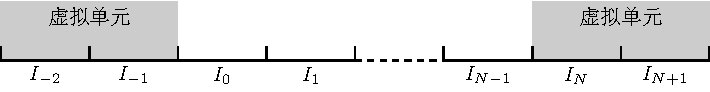
\includegraphics{fig/tikz/ghostcell.pdf}
  \caption{虚拟单元示意图。
  }
  \label{fig:1D-ghostcell}
\end{figure}

虚拟单元要根据边界条件赋值,
例如对于周期边界,
我们有
\begin{equation}
  {\bm u}_{m} = {\bm u}_{N-m}, \quad m<0, \quad
  {\bm u}_{N+m} = {\bm u}_{m}, \quad m\ge 0.
\end{equation}
对于狄利克雷边界,
有
\begin{equation}
  {\bm u}_{m} = {\bm u}_L, \quad m<0, \quad
  {\bm u}_{N+m} = {\bm u}_R, \quad m\ge 0.
\end{equation}
对于欧拉方程组的反射边界,
满足
\begin{equation}
  \begin{aligned}
     & {\rho}_{m} = {\rho}_{-1-m}, \quad
    {u}_{m} = -{u}_{-1-m}, \quad
    {p}_{m} = {p}_{-1-m}, \quad
     & m<0,                                  \\
     & {\rho}_{N+m} = {\rho}_{N-1-m}, \quad
    {u}_{N+m} = -{u}_{N-1-m}, \quad
    {p}_{N+m} = {p}_{N-1-m}, \quad
     & m\ge 0.
  \end{aligned}
\end{equation}
在二维情形下,
也有类似的结论。

\section{小结}

在本章,
我们发现原始的两步四阶时间推进框架的紧致性和高精度不可兼得。
如果导数重构采用更加紧致的埃尔米特重构,
那么所得格式在光滑区域的精度不超过三阶精度。
随后,
我们分析了其原因,
并提出了改进的两步四阶时间推进框架。
在改进的框架中导数重构采用更加紧致的埃尔米特重构时,
获得的数值格式可以在光滑区域保持四阶精度。
最后,
我们简单介绍了三步四阶时间推进框架和虚拟单元边界处理技术。

接下来,
我们将基于改进的两步四阶时间推进框架,
设计一种求解双曲守恒律的紧致两步四阶数值格式。